%\chapter[Search for the SM Higgs boson in the \boldmath$\hww$ channel with the first \boldmath$13\TeV$ LHC data]{Search for the SM Higgs boson in the \boldmath$\hww$ channel with the first \boldmath$13\TeV$ LHC data}\label{chap5}
\chapter[Measurement of Higgs boson production using \boldmath$\hww$ decays with first \boldmath$13\TeV$ data]{Measurement of Higgs boson production using \boldmath$\hww$ decays with first \boldmath$13\TeV$ data}\label{chap5}
\chaptermark{Measurement of Higgs boson production using \boldmath$H\to W^+W^-$ decays at \boldmath$13\TeV$}
\thispagestyle{empty}

In this chapter, the first measurement of the 125\GeV Higgs boson cross section times branching ratio to a W boson pair at 13\TeV is presented, using a total integrated luminosity of 2.3\ifb,
collected during the 2015 proton-proton data taking period of the LHC. The analysis strategy follows the one described in Chapter~\ref{chap4}, with some differences described in the following.

With respect to the centre-of-mass energy of 8\TeV, the ggH production cross section at 13\TeV is expected to increase of a factor of 2, thus raising the number of expected signal events. Nevertheless, the cross section of the background processes increases as well: in particular, the WW production cross section of a factor of 1.8 and the \ttbar cross section of a factor of 3.5.

%\section{Introduction}
%%%%%%%%%%%%%%%%%%%%%%%%%%%%%%%%%%%%%%%%%%%%%%%%%%%%%%%%%%%%%%%%%%%%%%
\label{sec:Introduction}
The discovery of a new boson consistent with the standard model (SM) Higgs boson has been reported by ATLAS and CMS Collaborations in 2012.
The discovery has been followed by a comprehensive set of studies of properties of this new boson in several production and decay channels and no evidence of deviation from the SM expectation has been found so far. The CMS studies in the \hwwllnn decay channel include the measurement of the Higgs properties, as well as constraints on the Higgs total decay width and gauge bosons anomalous couplings.

In this section the measurement of the transverse momentum spectrum of the Higgs boson, produced in proton-proton collisions at a center-of-mass energy of $\sqrt{s}=8$\TeV, is reported.
This measurement can be used to directly inspect the perturbative QCD theory in the Higgs sector.
In particular the $p_T^H$ variable is sensitive to the Higgs production mode and the differential distribution in this variable can be used to inspect the effects of the top quark mass in the gluon fusion top loop. Moreover, any observed deviation from the SM expectation, especially in the tail of the $p_T^H$ distribution, could be a hint of physics beyond the SM.\\
Similar measurements have already been performed by CMS and ATLAS experiments in the ZZ and $\gamma\gamma$ Higgs decay channels.
The measurement reported here is the first measurement of the Higgs \pt spectrum in the WW decay channel.\\
The cross section has been measured in a fiducial phase space defined using generator level variables in order to mimic the experimental acceptance and reduce the systematic uncertainties on the procedure of extrapolating the results in a larger phase space.\\
The Higgs transverse momentum has been reconstructed calculating the vector sum of the dilepton system transverse momentum plus missing transverse energy 
\begin{equation}
\vec{p}_\mathrm{T}^\mathrm{H} = \vec{p}_\mathrm{T}^{\ell\ell} + \vec{p}_\mathrm{T}^\mathrm{miss}
\end{equation}
The signal has been extracted subtracting all backgrounds by means of a binned Maximum Likelihood fit and has been then corrected for the efficiency of the analysis selections and for the detector resolution effects using an unfolding procedure.\\
The differential measurement has been performed in six bins of \pth with variable widths, chosen to have approximately the same purity in each bin, as explained in section \ref{sec:AnalysisStrategy}.\\




\section{Data and simulated samples}\label{chap5:dataset}

Data recorded in proton-proton collisions at 13\TeV during 2015 are used in the analysis, with a total integrated luminosity of 2.3\ifb. Single and double lepton triggers are used, similarly to the same analysis at 8\TeV. The HLT trigger \pt thresholds used in this analysis are listed in Table~\ref{tab:trigger13TeV}.

\begin{table}[htb]
\begin{center}
\caption{Transverse momentum thresholds required for lepton triggers at HLT level. 
         Double set of thresholds indicates the thresholds for each leg of the double lepton triggers.}
\begin{tabular}{ccc}
\toprule
Trigger path       & Threshold \\
\midrule
Single electron    & $\pt > 23$\GeV         \\  
Single muon        & $\pt > 20$\GeV         \\ 
Muon-Electron      & $\pt > 17$ and $12$\GeV         \\ 
Electron-Muon      & $\pt > 17$ and $8$\GeV         \\ 
\bottomrule
\end{tabular}
\label{tab:trigger13TeV} 
\end{center}
\end{table}

\begin{comment}
\begin{table}[h]
\caption{HLT paths related to Electrons}
\label{table:ele_trigg_13}
\scalebox{0.75}{
\begin{tabular}{ll}
\hline
HLT Path & Description \\
\hline\hline
HLT\_Ele23\_WPLoose\_Gsf\_v*   &
\parbox{11cm}{$\,$ \\Single Electron trigger. Best trigger to be used for 2015 data. In HWW, we are using ``Trigger safe'' Id. Turn on is at around Ele $\rm p_{T}$ = 30 GeV\\}\\
\hline
HLT\_Ele17\_Ele12\_CaloIdL\_TrackIdL\_IsoVL\_DZ\_v* &
\parbox{11cm}{$\,$ \\Double Electron Trigger. Best trigger to cover the turn on region from single electron trigger. ``DZ'' filter is also present. Its efficiency is also calculated separately.}\\
\hline
HLT\_Ele12\_CaloIdL\_TrackIdL\_IsoVL\_v* &
\parbox{11cm}{$\,$ \\This electron leg of \\
HLT\_Mu17\_TrkIsoVVL\_Ele12\_CaloIdL\_TrackIdL\_IsoVL\_v*\\
same as Ele12 leg of double electron trigger.\\} \\
\hline
HLT\_Ele17\_CaloIdL\_TrackIdL\_IsoVL\_v*&
\parbox{11cm}{$\,$ \\This electron leg of\\
HLT\_Mu8\_TrkIsoVVL\_Ele17\_CaloIdL\_TrackIdL\_IsoVL\_v* \\
same as Ele17 leg of double electron trigger.} \\
\hline
\end{tabular}
}
\end{table}

\begin{table}
\caption{Muon trigger's elements description}
\label{table:mu_trigg_13}
\scalebox{0.8}{
\begin{tabular}{ll}
\hline
HLT path \\
\hline\hline
HLT\_IsoMu18\_v*   & 
\parbox{11cm}{$\,$ \\single muon trigger\\}\\
\hline
HLT\_IsoTrMu20\_v* &
\parbox{11cm}{$\,$ \\single muon trigger with tracker isolation\\}\\
\hline
HLT\_Mu17\_TrkIsoVVL & 
\parbox{11cm}{$\,$ \\leg for the HLT\_Mu17\_TrkIsoVVL\_Mu8\_TrkIsoVVL\_DZ\_v*,\\
HLT\_Mu17\_TrkIsoVVL\_TkMu8\_TrkIsoVVL\_DZ\_v* and\\ 
HLT\_Mu17\_TrkIsoVVL\_Ele12\_CaloIdL\_TrackIdL\_IsoVL\_v*\\
double lepton triggers\\} \\
\hline
HLT\_Mu8\_TrkIsoVVL &
\parbox{11cm}{$\,$ \\leg for the HLT\_Mu17\_TrkIsoVVL\_Mu8\_TrkIsoVVL\_DZ\_v* and\\
HLT\_Mu8\_TrkIsoVVL\_Ele17\_CaloIdL\_TrackIdL\_IsoVL\_v* \\ 
double lepton triggers\\} \\
\hline
HLT\_TkMu8\_TrkIsoVVL &
\parbox{11cm}{$\,$ \\leg for the HLT\_Mu17\_TrkIsoVVL\_TkMu8\_TrkIsoVVL\_DZ\_v*\\
double muon trigger\\} \\
\hline
$DZ_{\mu\mu}$ &
\parbox{11cm}{$\,$ \\efficiency of DZ cut in \\
the HLT\_Mu17\_TrkIsoVVL\_Mu8\_TrkIsoVVL\_DZ\_v*\\
and HLT\_Mu17\_TrkIsoVVL\_TkMu8\_TrkIsoVVL\_DZ\_v* \\
double muon triggers, it is around 95\%\\} \\
\hline
\end{tabular}
}
\end{table}
\end{comment}

The trigger efficiencies are measured in data and applied to simulated events as described in Sec.~\ref{subsec:Datasets}.

%Monte Carlo
Concerning the simulated samples, several different MC generators are used. 
Higgs boson signal samples are simulated in all channels using \textsc{Powheg v2}~\cite{Nason:2004rx,Frixione:2007vw,Alioli:2010xd}, designed to describe the full NLO properties of these processes.
In particular, for Higgs boson produced via ggH~\cite{Alioli:2008tz}, and VBF~\cite{Nason:2009ai},
the decay into two W bosons and subsequently into leptons is done using \textsc{JHUGen} v5.2.5. 
For associated production with a vector boson ($\mathrm{W}^{+}\mathrm{H}$, $\mathrm{W}^{-}\mathrm{H}$, ZH)~\cite{Luisoni:2013kna}, including gluon fusion produced ZH (ggZH), 
the Higgs boson decay is instead simulated using \textsc{pythia} 8.1~\cite{Sjostrand:2007gs}. All the signal samples are generated assuming a Higgs boson mass of 125\GeV.

The \textsc{Powheg v2}~\cite{Melia:2011tj} is also used for simulating the $\mathrm{q\bar q}$ induced WW  production in different decay channels. The simulated events are reweighted to reproduce the $\pt^\mathrm{WW}$ distribution obtained from \pt-resummed calculations~\cite{Meade:2014fca,Jaiswal:2014yba}. Gluon fusion produced WW is generated at LO QCD accuracy using \textsc{mcfm} v7.0~\cite{Campbell:2013wga}.
%The cross section used for normalizing WW processes produced via $\mathrm{q\bar q}$ was computed at next-to-next-to-leading order (NNLO)~\cite{Gehrmann:2014fva}. 
%In order to control the top quark background processes, the analysis is performed with events that have no more than one high-\pt jet. The veto on high-\pt jets enhances the importance of logarithms of the jet \pt, spoiling the convergence of fixed-order calculations of the qq$\rightarrow$WW process and requiring the use of dedicated resummation techniques for an accurate prediction of differential distributions~\cite{Meade:2014fca,Jaiswal:2014yba}. The \pt of the jets produced in association with the WW system is strongly correlated with its transverse momentum, $\pt^\mathrm{WW}$, especially in the case where only one jet is produced. The simulated qq$\rightarrow$WW events are reweighted to reproduce the $\pt^\mathrm{WW}$ distribution from the \pt-resummed calculation.

The \ttbar process with dilepton final state is also generated using \textsc{Powheg v2}. The simulated processes for the WW and \ttbar production are illustrated in Table~\ref{tab:wwl}, together with the associated cross sections. Other minor background samples are also generated, a list of the most relevant ones is presented in Table~\ref{tab:otherbck}.

\begin{table}[htb]
\caption{Simulated processes for \ttbar and \WW production.}\label{tab:wwl}
\begin{center}
\begin{tabular}{lc}
\toprule
Process & $\sigma\times\mathcal{B}$ [pb] \\
\midrule
\ttbar$\rightarrow$WW$\mathrm{b\bar{b}}\rightarrow2\ell2\nu \mathrm{b\bar{b}}$ & 87.31 \\
$\mathrm{q\bar q}\rightarrow$WW$\rightarrow2\ell2\nu$ & 12.178 \\
$\mathrm{gg}\rightarrow$WW$\rightarrow2\ell2\nu$ & 0.5905 \\
%$gg\rightarrow$\WW$\rightarrow2\ell2\nu$ (H diagr.) & 0.9544\\
\bottomrule
\end{tabular}
\end{center}
\end{table}

\begin{table}[htb]
\caption{Simulated samples for other minor background processes used in the analysis. Single top quark production includes the dominant tW process, as well as the sub-dominant production in the s- and t-channels.\label{tab:otherbck}}
\begin{center}
\begin{tabular}{lc}
\toprule
Process & $\sigma\times\mathcal{B}$ [pb] \\
\midrule
Single top &   71.7  \\
Drell-Yan ($10\GeV < \mll < 50\GeV$)  &  20471.0  \\
Drell-Yan ($\mll > 50\GeV$)   &  6025.26  \\
WZ$\to2\ell2\mathrm{q}$ &  5.5950 \\
ZZ$\to2\ell2\mathrm{q}$ &  3.2210 \\
WWZ &  0.1651 \\
WZZ &  0.05565 \\
ZZZ &  0.01398  \\
\bottomrule
\end{tabular}
\end{center}
\end{table}

All processes are generated using NNPDF2.3~\cite{Ball:2013hta,Ball:2011uy} for NLO generators.
The LO version of the same PDF set is used for LO generators. All the event generators are interfaced  to \textsc{pythia} 8.1~\cite{Sjostrand:2007gs} for the showering of
partons and hadronization, as well as including a simulation of the underlying event (UE) and multiple interaction (MPI) based on the CUET8PM1 tune~\cite{Khachatryan:2015pea}. 

To estimate the systematic uncertainties related to the choice of UE and MPI tune, the signal processes and the WW background are also generated with two alternative tunes which are representative of the errors on the tuning parameters.
The showering and hadronization systematic uncertainty is estimated by interfacing the same MC samples with the \textsc{herwig++} 2.7 parton shower~\cite{Richardson:2013nfo,Bellm:2013hwb} instead of \textsc{pythia 8}.

Drell-Yan (DY) production of Z/$\gamma^{*}$ is generated using \textsc{amc@nlo}~\cite{Alwall:2014hca}. 
Other multiboson processes, such as WZ,ZZ, and VVV (V$=$W/Z), are generated with \textsc{amc@nlo} and normalized to the cross section calculation at NLO accuracy.

The simulated samples are generated with distributions for the number of pile-up interactions that are meant to roughly cover, though not exactly match, the conditions expected for the different data-taking periods. In order to factorize these effects, the number of true pile-up interactions from the simulation truth is reweighted to match the data.
In Fig.~\ref{Fig:pu}, the effect of this reweighting on a sample enriched in Drell-Yan events is shown. The average number of pile-up is approximately $11.5$.

\begin{figure}[htbp]
\centering
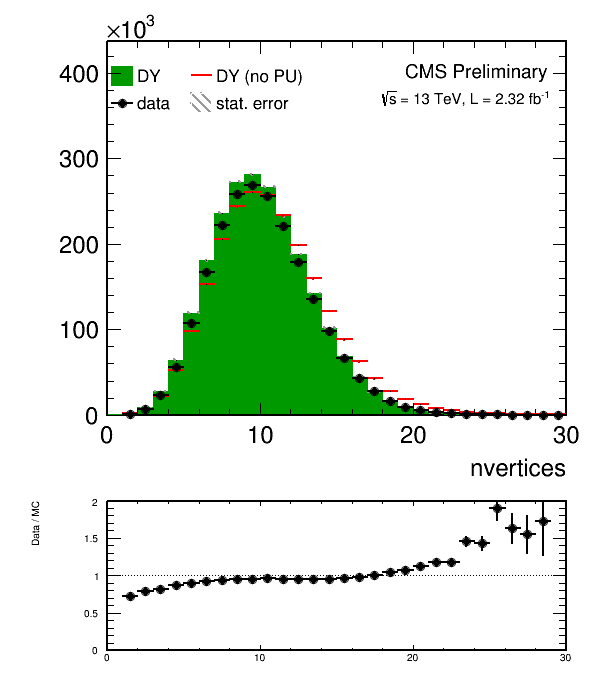
\includegraphics[width=0.45\textwidth]{images/13TeV/nvertices.png}
\caption{
    Distribution of the number of vertices in a Drell-Yan enriched phase space in data,
    together with the simulation before (red) and after (solid green) the pile-up reweighting.}
    \label{Fig:pu}
\end{figure}

For Higgs boson signal, the inclusive cross sections used are the ones reported by the LHC Higgs Cross Section Working Group~\cite{temphiggsxsecs}. The ggH cross section is computed at NNLO+NNLL QCD and NLO EW accuracy, while NNLO QCD and NLO EW accuracy is used for the other production modes. The branching fractions are the ones reported in Ref.~\cite{Heinemeyer:2013tqa}.

The cross section used for the $\mathrm{q\bar q}$ induced WW processes is computed at NNLO QCD accuracy~\cite{Gehrmann:2014fva}. The normalization of this background is eventually directly taken from a fit to data and the NNLO cross section is used just as an initial guess. The LO cross section for the gluon induced WW process is obtained directly from \textsc{mcfm}, and a $k$-factor of 1.4 is applied to correct for the difference between the LO and NLO theoretical calculation~\cite{Caola:2015rqy}.
The contribution of the interference between the $\mathrm{gg \to WW}$ and $\mathrm{gg\to H\to WW}$ processes is also evaluated using \textsc{mcfm} and is found to be negligible compared to the signal contribution.

The cross sections of the different single top processes are estimated by the LHC Top Working group~\cite{singletop} with NLO accuracy.
The \ttbar cross section is also provided by the LHC Top Working group~\cite{topxsec}, and it is computed at NNLO accuracy, with NNLL soft gluon resummation.


\section{Analysis strategy}\label{chap5:analysis_strategy}

\subsection{Event reconstruction}

Regarding electrons, muons, jets and \MET definition and reconstruction, the standard CMS recommendations described in Chapter~\ref{chap2} are used. The specific selections used in this analysis are briefly summarized below.

Muons are identified according to the definition described in Sec.~\ref{sec:muID}, with some specific modifications regarding the impact parameters of the tracks with respect to the primary vertex. In particular the requirements are lowered to $d_{xy}<0.01$\,cm and $d_z < 0.1$\,cm with respect to the \emph{tight muon selection} illustrated in Table~\ref{tab:tightmuon}.

%\begin{itemize}
%\item identified by the standard medium muon selection described in Sec.~\ref{sec:Objects}; \textcolor{red}{Not yet defined :)}
%\item $\pt> 10$\GeV;
%\item $|\eta < 2.4|$;
%\item $|d_{xy}| < 0.01$\,cm for $\pt < 20$\GeV and $|d_{xy}| < 0.02$\,cm for $\pt > 20$\GeV, $d_{xy}$ being the transverse impact parameter with respect to the primary vertex;
%\item $|d_{z}| < 0.1$\,cm, where $d_z$ is the longitudinal distance of the muon track in the tracker extrapolated along the beam direction.
%\end{itemize}

The PF relative isolation described in Eq.\eqref{eq:isomu} is used for muon isolation, corresponding to a requirement on the isolation variable of $I^{rel}_{\Delta\beta} < 0.15$. In addition a tracker relative isolation is also applied.

The tight working point described by the requirements in Table~\ref{tab:tightele} is used for the electron identification. Some additional requirements to make the selection ``trigger-safe'' are included. This is done because the electron triggers already include some identification and isolation requirements that are based on the raw detector information, while the offline selections make use of particle flow requirements. The ``trigger-safe'' selections are defined to make the offline identification and isolation requirements tighter with respect to the online triggers.

The simulated events are corrected for the lepton trigger, identification and isolation efficiencies measured in data using the same techniques described in Sec.~\ref{sec:Selections}.

Jets are obtained clustering the particle flow objects using the anti-$k_t$ algorithm with a distance parameter of 0.4. The CHS pile-up mitigation technique is used and the jet energy corrections are applied, as described in Sec.~\ref{sec:jec}. 
To reject jets arising from calorimeter or readout electronics noise, the loose working point for PF jet identification is used (see Sec.~\ref{sec:jetID}). The jet counting used in the event selection is based on jets with $\pt>30$\GeV.

\subsection{B tagging performance}

The b tagging algorithm is chosen comparing the performance of different algorithms on simulated \hwwllnn signal produced via the ggH mechanism and \ttbar background.

The b veto efficiency, $\epsilon_\text{b veto}$, is computed separately for the two samples and for various b tagging algorithms. To compare the b tagging performance, $\epsilon_\text{b veto}$ is computed for different working points, i.e. different selections on the specific b tagging discriminator, and the results are reported in the form of a ROC curve. In general, ROC curves are built reporting the signal efficiency on the $x$ axis and the background rejection on the $y$ axis. In this case the $x$ axis shows the b-jets veto efficiency for signal ($\epsilon_\text{b veto}^\text{ggH}$) and the $y$ axis the \ttbar background rejection ($1-\epsilon_\text{b veto}^{\ttbar}$). The best algorithm is the one that provides the highest background rejection for a given signal efficiency. 

The ROC curves corresponding to events with 0, 1 and $\geq 2$ jets are shown in Fig.~\ref{fig:btag}. Events considered for this study are the ones related to the typical \hww phase space. Here 0 jets means that events do not contain any jet with \pt above 30\GeV. In this category the b veto rejects the event if at least one jet with $20\GeV < \pt < 30\GeV$ is identified by the b tagging algorithm. Events containing exactly one jet with $\pt>30$\GeV are rejected if that jet is b-tagged, while events with 2 or more jets are rejected if at least one jet is b-tagged.

\begin{figure}[htb]
\centering
\subfigure[$N_\mathrm{jets} = 0$]{
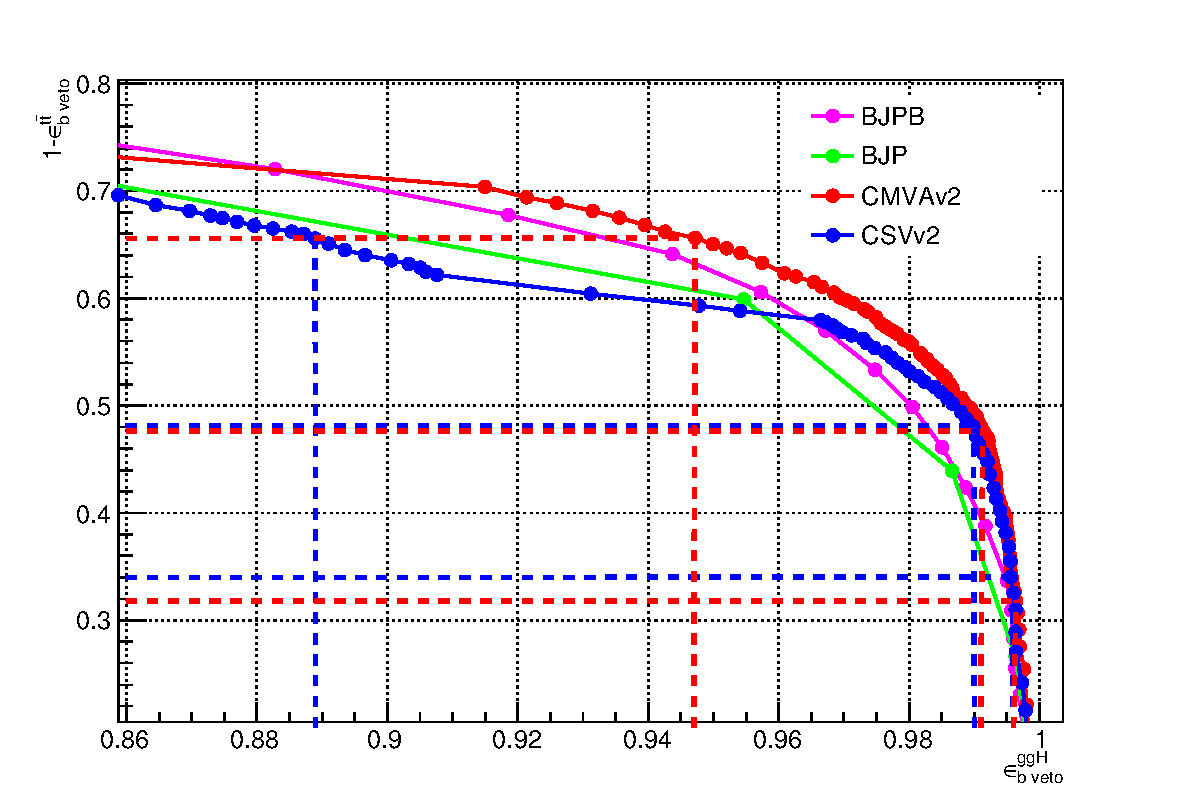
\includegraphics[width=0.45\textwidth]{images/13TeV/ROC_njet0.pdf}
}
\subfigure[$N_\mathrm{jets} = 1$]{
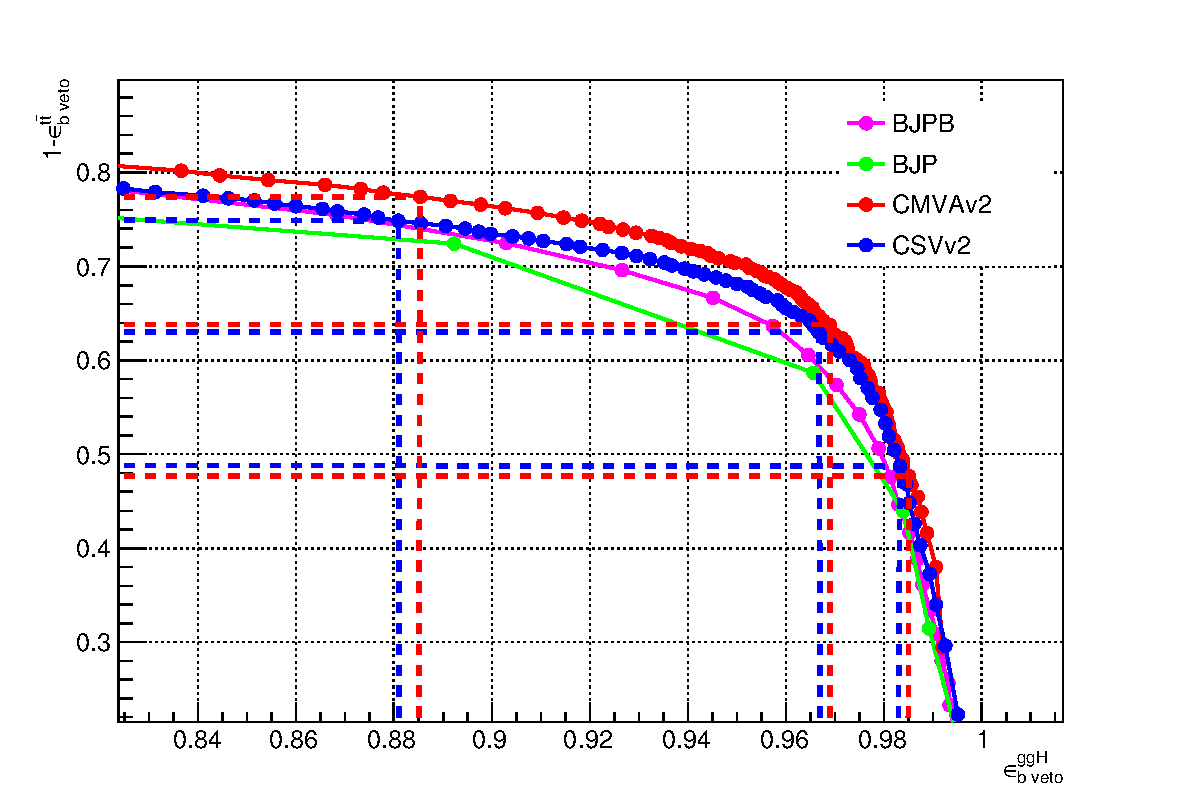
\includegraphics[width=0.45\textwidth]{images/13TeV/ROC_njet1.pdf}
}
\subfigure[$N_\mathrm{jets} \geq 2$]{
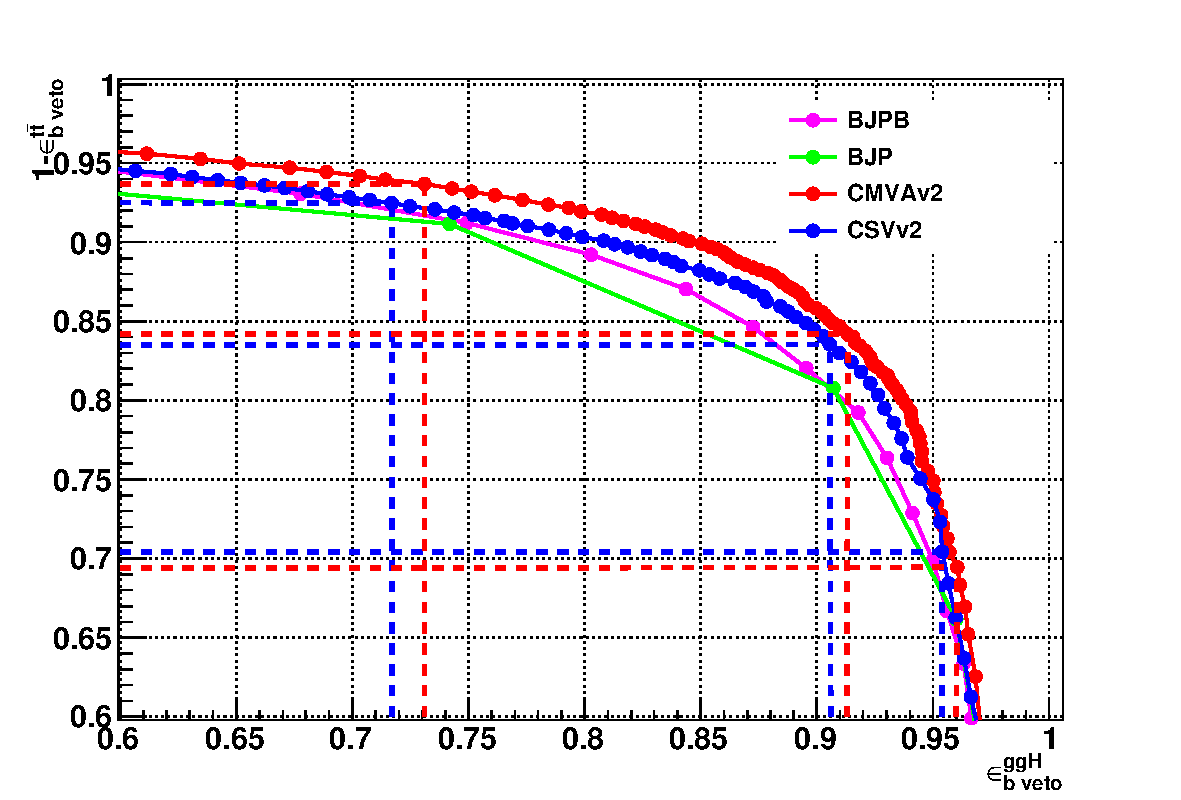
\includegraphics[width=0.45\textwidth]{images/13TeV/ROC_njetge2.pdf}
}
\caption{ROC curve for the b veto efficiency on signal and background events. The blue and red lines point out the signal efficiency and the background rejection corresponding to the three working points considered for the CSVv2 and the cMVAv2 algorithms
respectively.}\label{fig:btag}
\end{figure}

The ROC curves show that the cMVAv2 algorithm has the best performance for the analysis phase space among the algorithms taken into account. For both the CSVv2 and cMVAv2 algorithms\footnote{The CSVv2 and cMVAv2 algorithms are improved versions of the CSV and cMVA described in Sec.~\ref{sec:btag}, developed by CMS for the 13\TeV data taking period.}, three working points are defined corresponding to the mistag rates (see Sec.~\ref{sec:btag}) of 10\% (loose), 1\% (medium) and 0.1\% (tight). These mistag rates correspond roughly to $1-\epsilon_\text{b veto}^\text{ggH}$ in events with 1 jet. The distribution of the cMVAv2 discriminator associated to the leading jet for both the ggH and \ttbar samples is shown in Fig.~\ref{fig:discriminator}. The events falling on the left side of the vertical lines, which corresponds to the three working points of the cMVAv2 algorithm, are those that pass the b veto requirement.

\begin{figure}[htb]
\centering
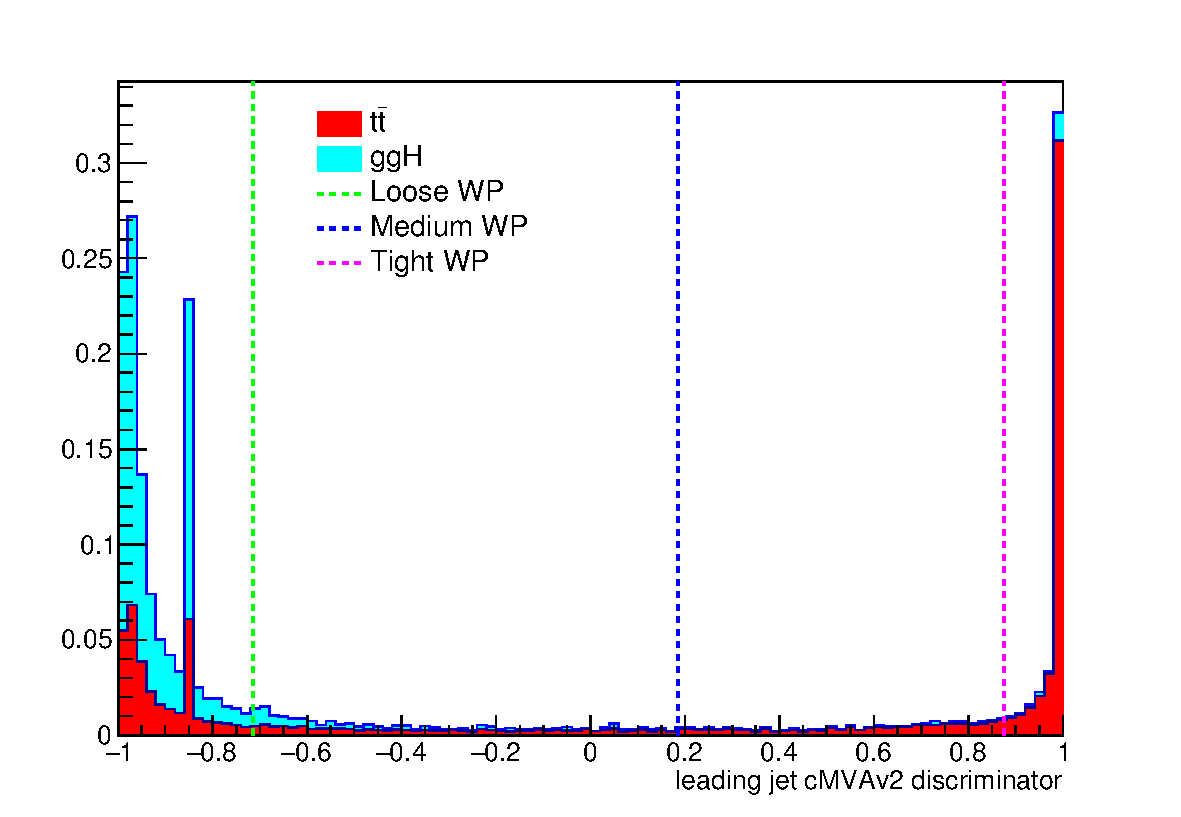
\includegraphics[width=0.6\textwidth]{images/13TeV/cmva_WP.pdf}
\caption{cMVAv2 discriminator associated to the leading jet (with $\pt > 30$\GeV) for both the ggH and the \ttbar processes. The two processes are normalized to unity and stacked. The vertical dashed lines show the discriminator value corresponding to the three working points.}\label{fig:discriminator}
\end{figure}

In order to determine the best working point for this analysis a signal significance assessment is performed, in which only statistical uncertainties are taken into account. The expected signal significance is calculated applying the event selections and using the statistical procedure described in the next sections, testing the effect of the b veto for the three working points.
The signal significance is computed for the two jet categories separately and eventually for the combination of the two. This leads to the values listed in Table~\ref{tab:significance_wp_combine} for the three working points. The loose working point is found to be the one for which the best signal significance is achieved in the combined $0+1$ jets category, and is thus chosen for the definition of the b veto requirement.

\begin{table}
\caption{Signal significance corresponding to the three working points of the cMVAv2 algorithm and for
different jet categories.\label{tab:significance_wp_combine}}
\begin{center}
\begin{tabular}{lccc}
\toprule
Jet category & Loose WP (-0.715) & Medium WP (0.185) & Tight WP (0.875) \\
\midrule
0 jets & 2.022 & 2.043 & 2.036 \\
1 jet & 1.439 & 1.404 & 1.305 \\
$0+1$ jets & 2.481 & 2.479 & 2.420 \\
\bottomrule
\end{tabular}
\end{center}
\end{table}

To correct for a possible different b tagging efficiency in data and simulation, the simulated events are reweighted using scale factors computed in bins of the jet $\eta$ and \pt.
The scale factors related to the b tagging efficiency and mistag rate, together with the corresponding uncertainties, are estimated in data and simulation adopting a Tag and Probe technique similar to the one described in Sec.~\ref{sec:ScaleFactors}.

The efficiency in simulation has to be computed for different jet flavours, i.e. b, c and light (u, d, s), using jet matching information\footnote{There are different techniques developed by the CMS Collaboration to assess the flavour of a reconstructed jet in simulation. The technique used here makes use of the flavour of the hadrons clustered into a jet.}.
The efficiencies for tagging b-, c- and light-jets estimated using simulated \ttbar events are shown in Fig.~\ref{fig:effmc} in $\eta$ and \pt bins. The uncertainties associated to the efficiencies are representative of the statistics of the simulated \ttbar sample, and are computed according to a binomial distribution.

\begin{comment}
These scale factors and the corresponding uncertainties are centrally calculated for each working point, in such a way to be employable by all the CMS analyses. The prescription to reweight the simulated events is the following. First of all one has to compute the b tagging efficiency using the MC samples, $\varepsilon_\mathrm{MC}(p_\mathrm{T}, \eta, f)$, for the chosen working point in bins of jet \pt and $\eta$. The efficiency has to be computed for different flavours $f$ of the jets, b, c and light (u,d,s), using the jet matching information\footnote{There are a couple of techniques developed by the CMS Collaboration to assess the flavour of a reconstructed jet in simulation. The technique used here makes use of the flavour of the hadrons clustered into a jet.} which is available in all the MC samples. An MC-based event weight is then calculated computing the probability $P_\mathrm{MC}$ of a given b tagging configuration to occur, e.g.:
\begin{equation}
P_\mathrm{MC}=\prod_{i~\in{}~b-tagged-jets}\varepsilon_{\mathrm{MC}_{i}}\prod_{j~\in{}~non-b-tagged-jets}(1-\varepsilon_{\mathrm{MC}_{j}})
\label{eq:btagpmc}
\end{equation}
Afterwards, a similar probability is computed using data:
\begin{equation}
P_\mathrm{DATA}=\prod_{i~\in{}~b-tagged-jets}SF_{i}\varepsilon_{\mathrm{MC}_{i}}\prod_{j~\in{}~non-b-tagged-jets}(1-SF_{j}\varepsilon_{\mathrm{MC}_{j}}) \quad ,
\label{eq:btagpdata}
\end{equation}
where $SF_{i}$ is the provided scale factor value for the relevant jet flavour, \pt and $\eta$. Products in Eqs.~\ref{eq:btagpmc} and \ref{eq:btagpdata} run over all jets. The event weight is finally given by the ration $P_\mathrm{DATA}/P_\mathrm{MC}$.

The b tagging efficiencies to be fed into Eq.~\ref{eq:btagpmc} and
Eq.~\ref{eq:btagpdata} are derived using \ttbar simulated events and applying basic leptonic
selections. These efficiencies are shown in Fig.~\ref{fig:effmc} for light
(a), c-jets (b) and b-jets (c), in bins of $\eta$ and \pt. The uncertainties associated to the efficiencies are representative of the statistics of the simulated \ttbar sample, and are computed according to a binomial distribution.
\end{comment}
\begin{figure}[!h]
\centering
\subfigure[]{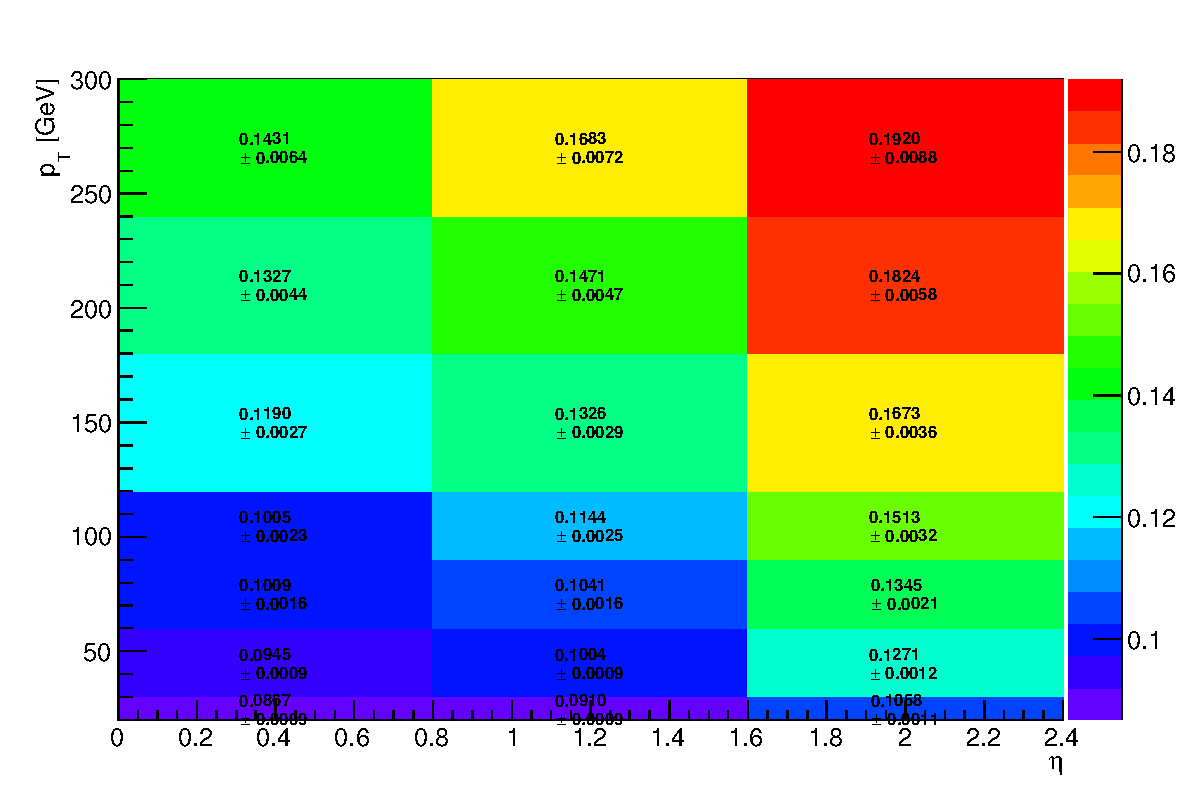
\includegraphics[width=0.4\textwidth]{images/13TeV/ljet_effmc-v2.pdf}}
\subfigure[]{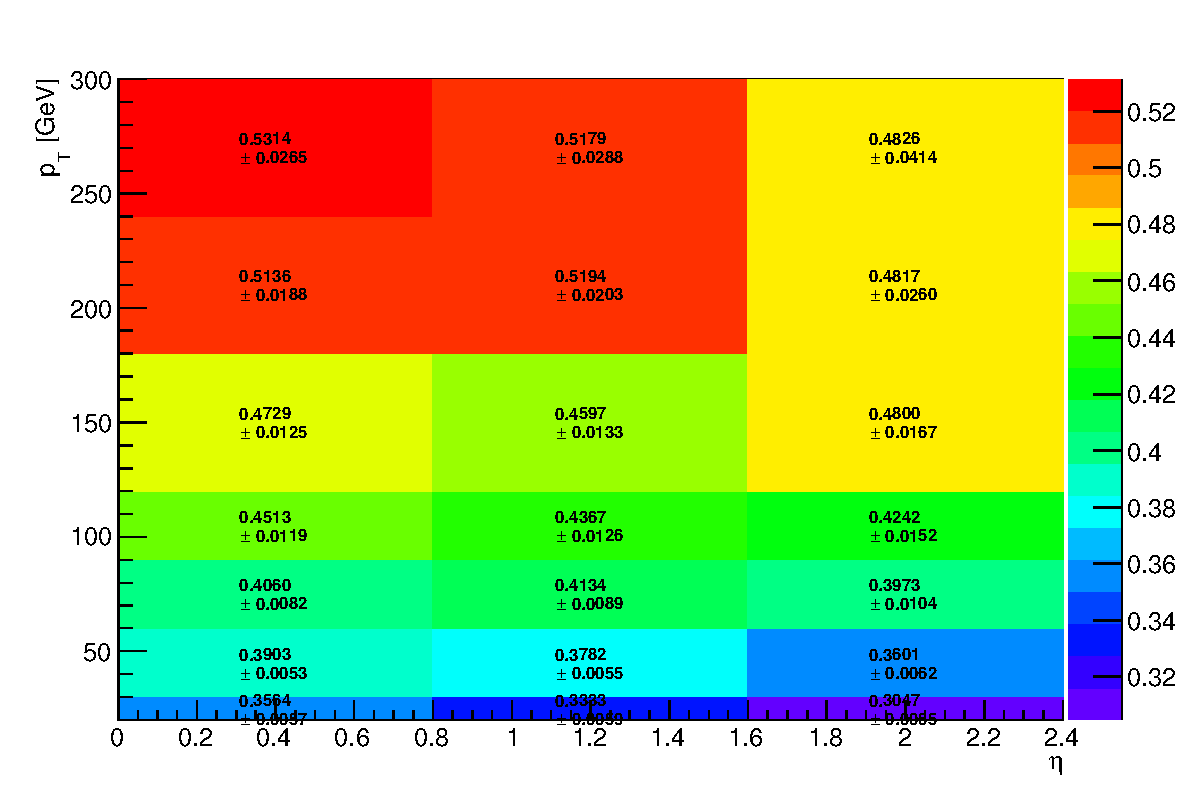
\includegraphics[width=0.4\textwidth]{images/13TeV/cjet_effmc-v2.pdf}}\\
\subfigure[]{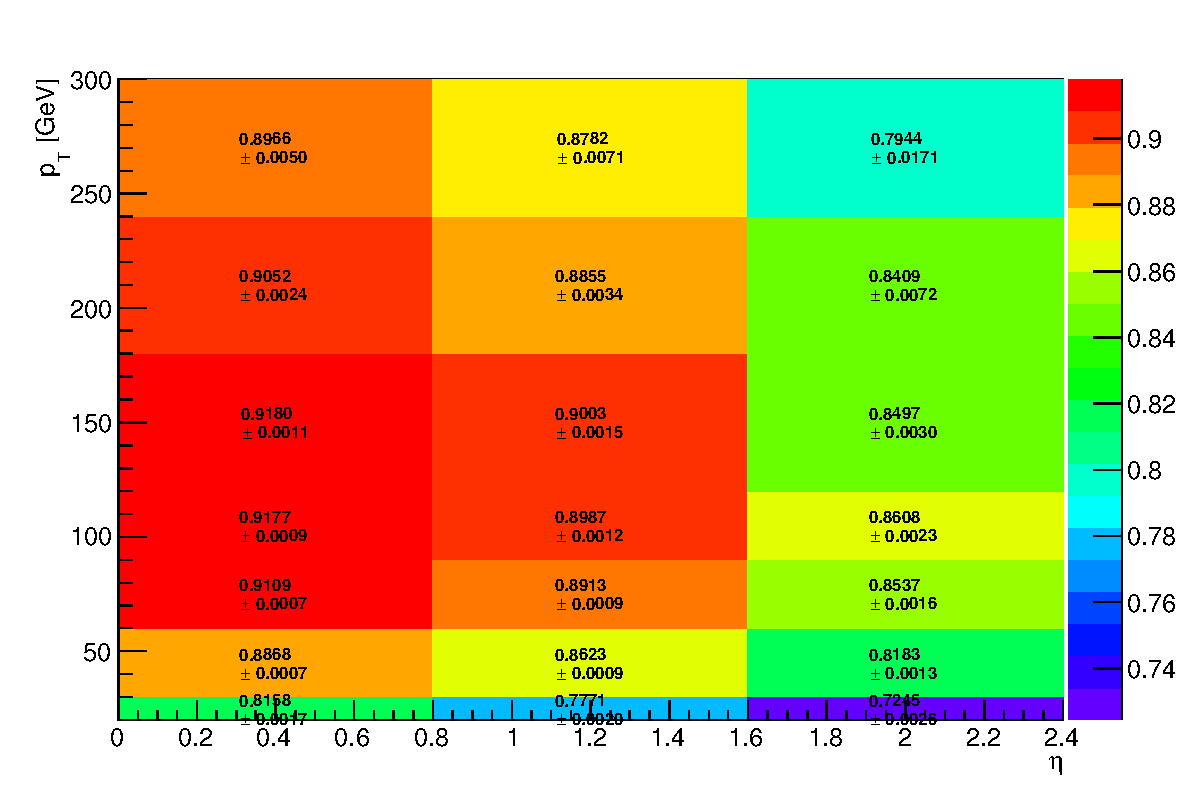
\includegraphics[width=0.4\textwidth]{images/13TeV/bjet_effmc-v2.pdf}}
\caption{B tagging efficiencies for light jets (a), c-jets (b) and
b-jets (c), as a function of $\eta$ and \pt.\label{fig:effmc}}
\end{figure}

The effect of the event reweighting is to correct the shape of the b tagging discriminator in simulation, moving events from the b tag region (discriminator greater than $-0.715$) to the b veto region (discriminator $ < -0.715$) and viceversa. A data/simulation comparison of the b tagging discriminator for the leading and subleading jets is performed to check the agreement after the application of the event weights. In order to evaluate the data/simulation agreement for b-jets, the data and simulation are compared to each other in a top quark enriched control region, defined by the following requirements:
\begin{itemize}
\item two leptons, an electron and a muon with opposite charge, with
leading lepton \pt greater than 20\GeV and subleading lepton \pt greater than 15\GeV;
\item no other electron or muon with \pt greater than 10\GeV;
\item \mll greater than 50\GeV;
\item at least two jets with \pt greater than 30\GeV;
\item at least one of the two leading jets with cMVAv2 b tagging score
greater than -0.715 (loose working point).
\end{itemize}
In order to evaluate the agreement for light jets, a second
control region is defined, populated by Z+light jet events, defined as follows:
\begin{itemize}
\item two electrons or two muons with opposite charge, with
leading lepton \pt greater than 20\GeV and subleading lepton \pt greater than 15\GeV;
\item no other electron or muon with \pt greater than 10\GeV;
\item \mll between 80\GeV and 110\GeV;
\item at least two jets with \pt greater than 30\GeV;
\item no jets above 20\GeV with a TCHE score above 2.1. 
\end{itemize}
Although the Z+jets sample is dominated by light flavor jets, a b-veto on an
alternative algorithm (TCHE) is applied to reduce the contamination from b-jets,
especially above the cMVAv2 cut. This helps mitigating possible discrepancies between data and simulation in the modelling of the heavy/light flavour ratio.
The comparison of the discriminator shape in data and simulation after the event reweighting is shown in Figs.~\ref{fig:bpogSF} and \ref{fig:bpogSF_Z} for the b-jets and light jets enriched control regions, respectively. The discriminator distribution is displayed in two bins and the edge represents the discriminator cut, in this case the one corresponding to the loose working point. Therefore, the entries falling in the left (right) bin correspond to events in which the leading or subleading jet fails (passes) the b tagging selection.

\begin{figure}[htb]
\centering
\subfigure[]{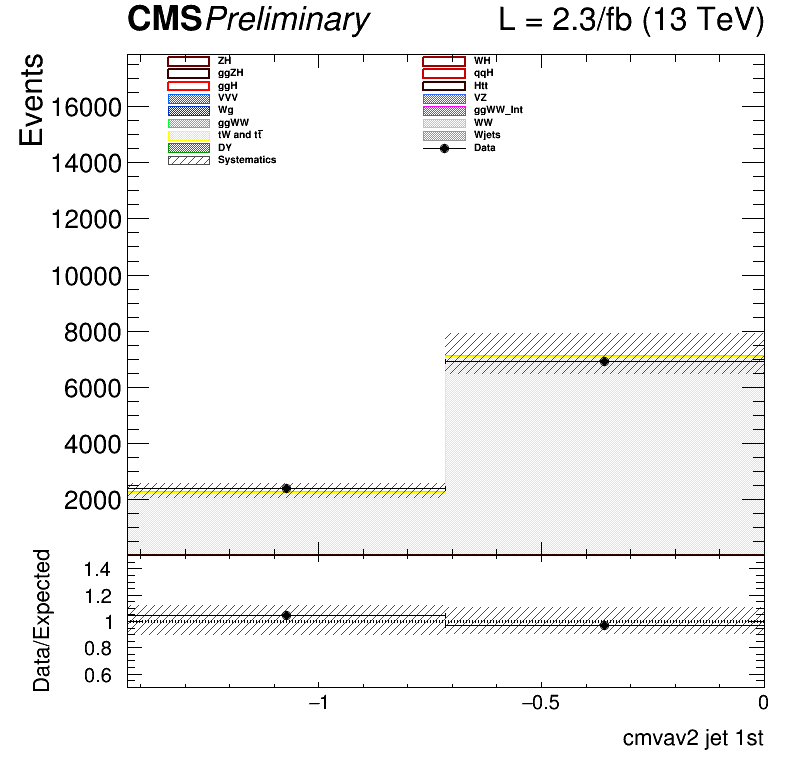
\includegraphics[width=0.4\textwidth]{images/13TeV/cratio_hww2l2v_13TeV_top_of1j_cmva_twobins_1.png}}
\subfigure[]{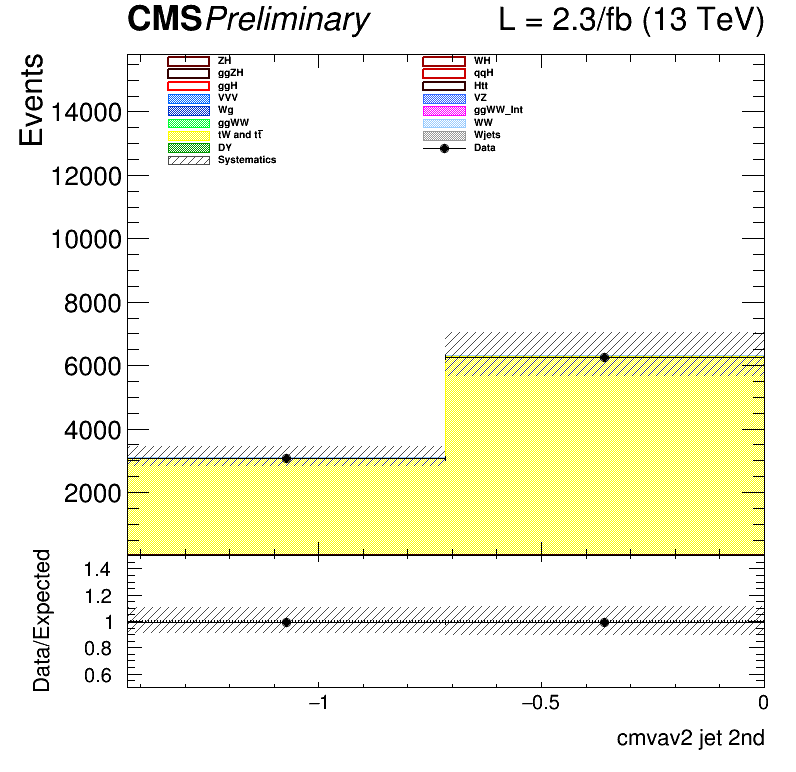
\includegraphics[width=0.4\textwidth]{images/13TeV/cratio_hww2l2v_13TeV_top_of1j_cmva_twobins_2.png}}
\caption{cMVAv2 discriminator for the leading (a) and subleading (b)
jet in the b-jets enriched control region.\label{fig:bpogSF}}
\end{figure}
\begin{figure}[htb]
\centering
\subfigure[]{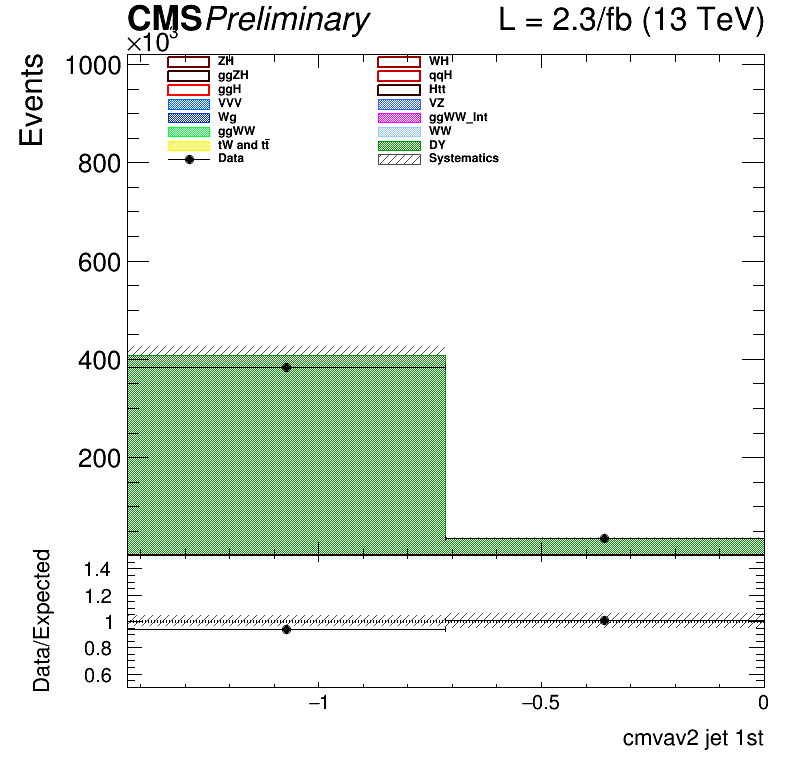
\includegraphics[width=0.4\textwidth]{images/13TeV/cratio_ZjetsCutTCHE_mumu_cmva_twobins_1.png}}
\subfigure[]{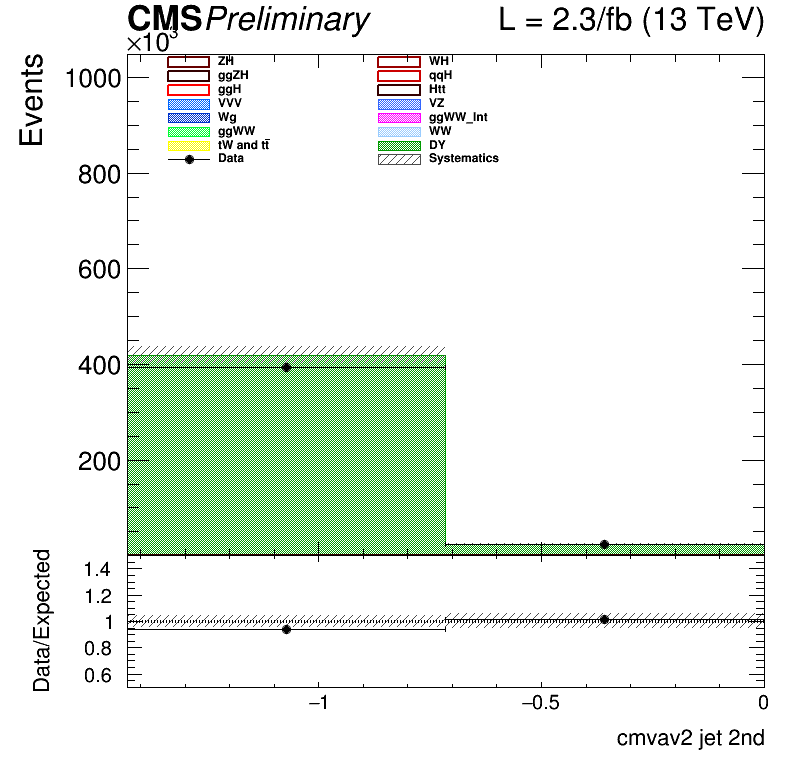
\includegraphics[width=0.4\textwidth]{images/13TeV/cratio_ZjetsCutTCHE_mumu_cmva_twobins_2.png}}
\caption{cMVAv2 discriminator for the leading (a) and subleading (b)
jet in the light jets enriched control region.\label{fig:bpogSF_Z}}
\end{figure}




\subsection{Event selection and background rejection}\label{chap5:eventSel}

Since the ggH production mechanism, which is the main production mode for a Higgs boson mass of 125\GeV, is characterized by the emission of few jets arising from initial state radiation, this analysis is limited to events with no jets or one jet. Higher jet multiplicity categories that are sensitive to other Higgs boson production mechanisms, such as VBF, are not included given the very low expected yield for the analysed integrated luminosity. 

Due to the large \dyll background in events with two electrons or two muons, only the $e\mu$ final state is studied in this early Run 2 data analysis, including the indirect contribution from $\tau$ leptons decaying to electrons or muons.
Exactly one electron and one muon with opposite charge and a minimum \pt of 10 (13)\GeV for the muon (electron) are required to be reconstructed in the event. One of the two leptons should also have a \pt larger than 20\GeV and both leptons are required to be well identified and isolated to reject fake leptons and leptons coming from hadron decays. To suppress background processes with three or more leptons in the final state, such as ZZ, WZ, Z$\gamma$, W$\gamma$, or triboson production, no additional identified and isolated lepton with $\pt>10$\GeV should be reconstructed. The low \mll region dominated by hadron decays of leptons is not considered in the analysis and \mll is requested to be larger than 12\GeV. To suppress the \dytt background where the $\tau$ leptons subsequently decay to an $e\mu$ final state, and suppress processes without genuine \MET, a minimal \MET of 20\GeV is required. The \dytt background is further reduced by requesting $\ptll > 30$\GeV. Finally the contribution from leptonic decays of single top quark and \ttbar production is reduced by requesting the b-jet veto.

The requirements described above define the WW baseline selection. After those requirements the data sample is dominated by events arising from the nonresonant WW production and \ttbar production. To further reduce the effect of these backgrounds on the signal sensitivity, the events are categorized depending on the jet multiplicity, counting jets with $\pt > 30$\GeV. Events with 0 associated jets mainly arise from WW production, while \ttbar production has a larger contribution in the category with 1 jet. The b-jet veto acts differently in the two categories as explained in the previous section: in the 0 jets category it rejects events containing at least one b-tagged jet with $20\GeV < \pt < 30\GeV$, while in the category with exactly one jet, the event is rejected if that same jet is identified by the b tagging algorithm.

Distributions of some variables of interest for the 0 and 1 jets categories are shown in Figs.~\ref{fig:distr1}, \ref{fig:distr2} and \ref{fig:distr3} after applying the WW baseline selections, with the addition of a cut on \mll to remove the Higgs signal contribution ($\mll > 80$\GeV), and a cut on \mt ($\mt > 60$\GeV) to define a phase space orthogonal to the control region used to estimate the \dytt background.

\begin{figure}
\centering
\subfigure[0 jets - $\pt^{\ell,1}$]{
  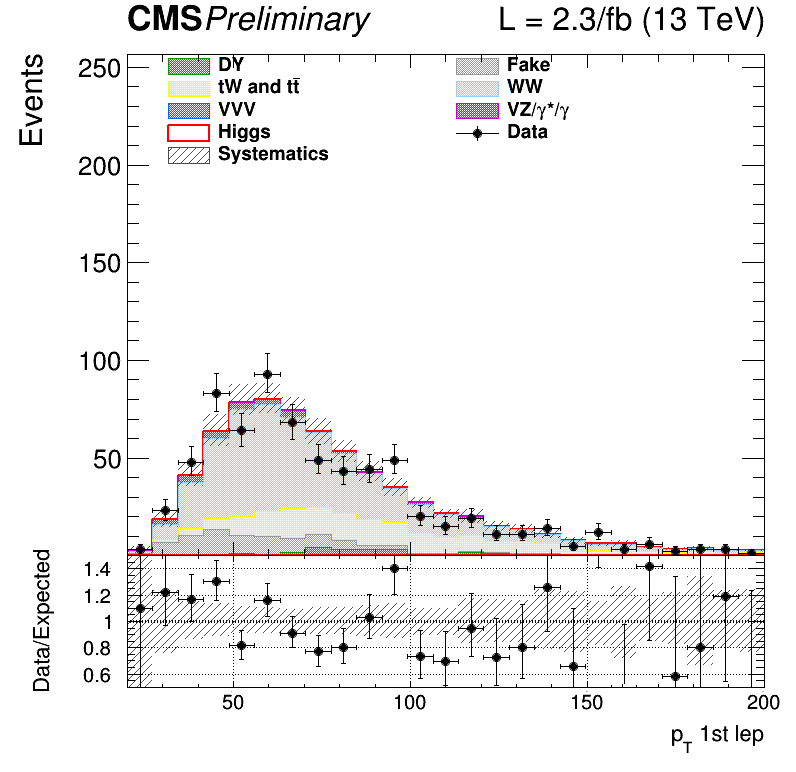
\includegraphics[width=0.45\textwidth]{images/13TeV/cratio_ww2l2v_13TeV_ww_of0j_pt1}
}
\subfigure[0 jets - $\eta^{\ell,1}$]{
  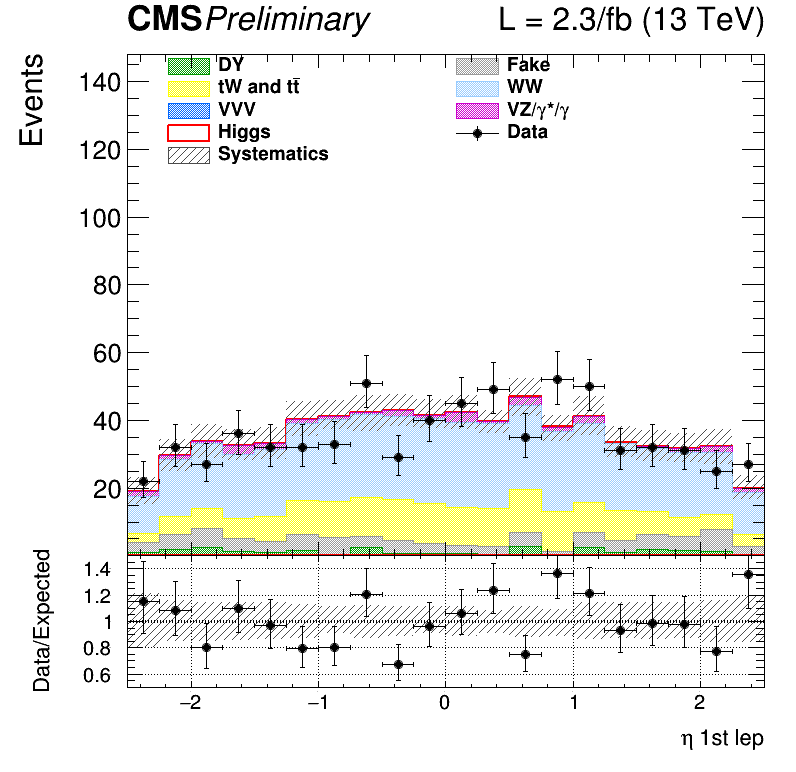
\includegraphics[width=0.45\textwidth]{images/13TeV/cratio_ww2l2v_13TeV_ww_of0j_eta1}
}\\
\subfigure[1 jet - $\pt^{\ell,1}$]{
  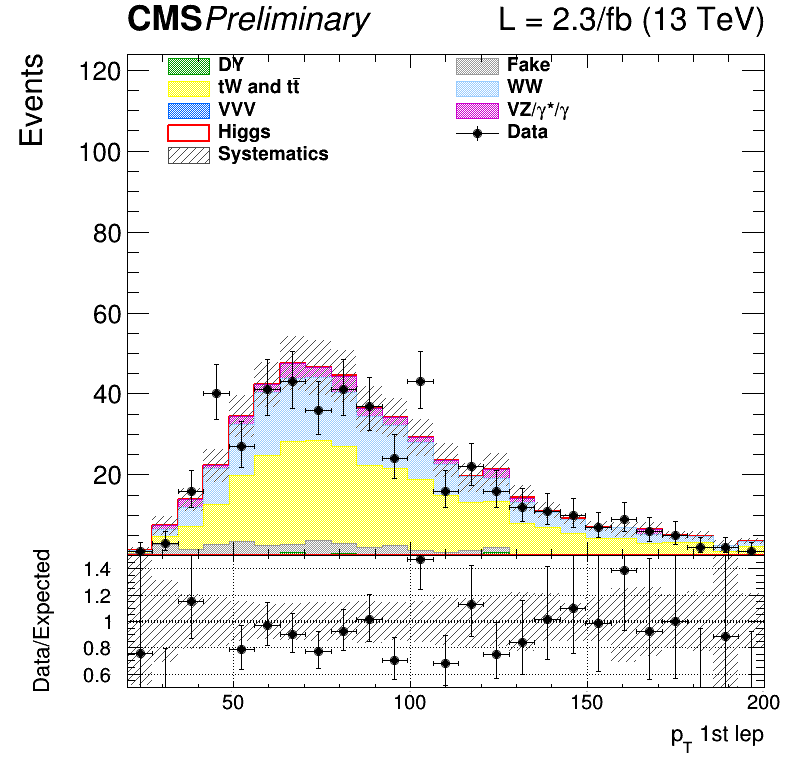
\includegraphics[width=0.45\textwidth]{images/13TeV/cratio_ww2l2v_13TeV_ww_of1j_pt1}
}
\subfigure[1 jet - $\eta^{\ell,1}$]{
  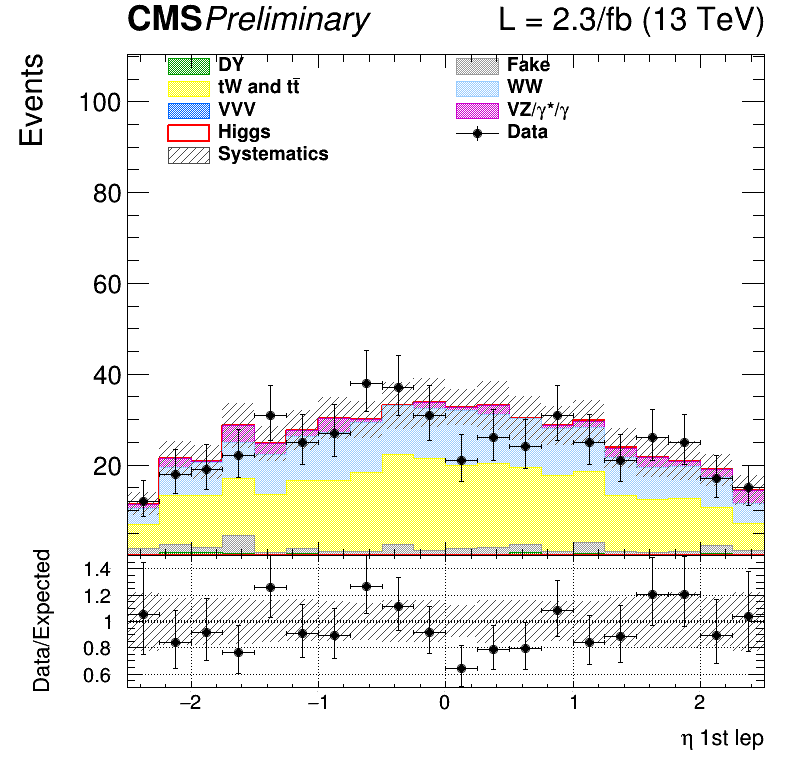
\includegraphics[width=0.45\textwidth]{images/13TeV/cratio_ww2l2v_13TeV_ww_of1j_eta1}
}
\caption{Distributions of \pt (left) and $\eta$ (right) of the leading lepton in events with 0 jets (upper row) and 1 jet (bottom row), for the main backgrounds (stacked histograms), and for a SM Higgs boson signal with $m_\mathrm{H}=125$\GeV (superimposed and stacked red histogram)  after the analysis event selection.}\label{fig:distr1}
\end{figure}

\begin{figure}
\centering
\subfigure[0 jets - $\pt^{\ell,2}$]{
  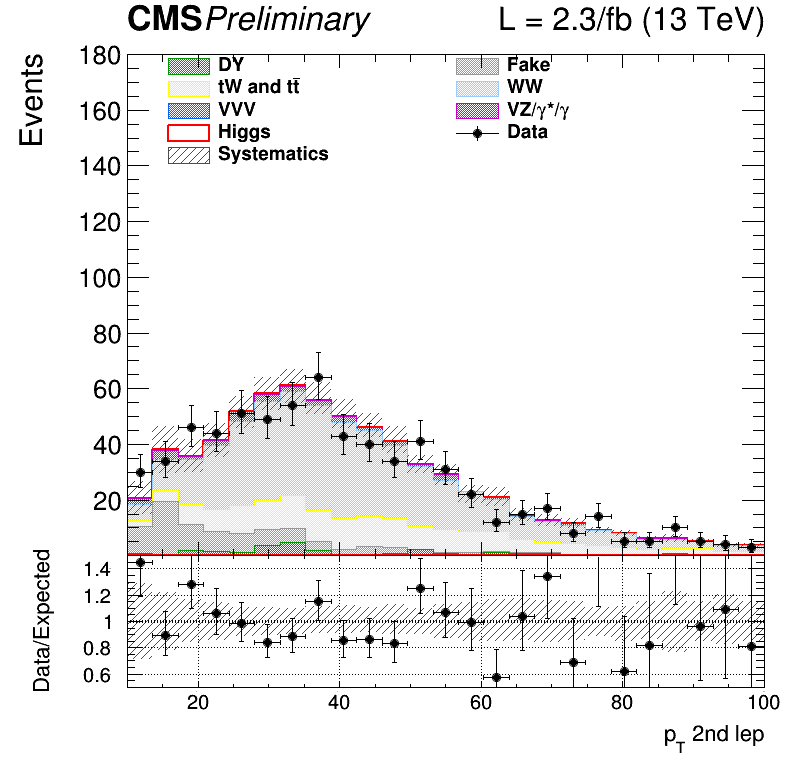
\includegraphics[width=0.45\textwidth]{images/13TeV/cratio_ww2l2v_13TeV_ww_of0j_pt2}
}
\subfigure[0 jets - $\eta^{\ell,2}$]{
  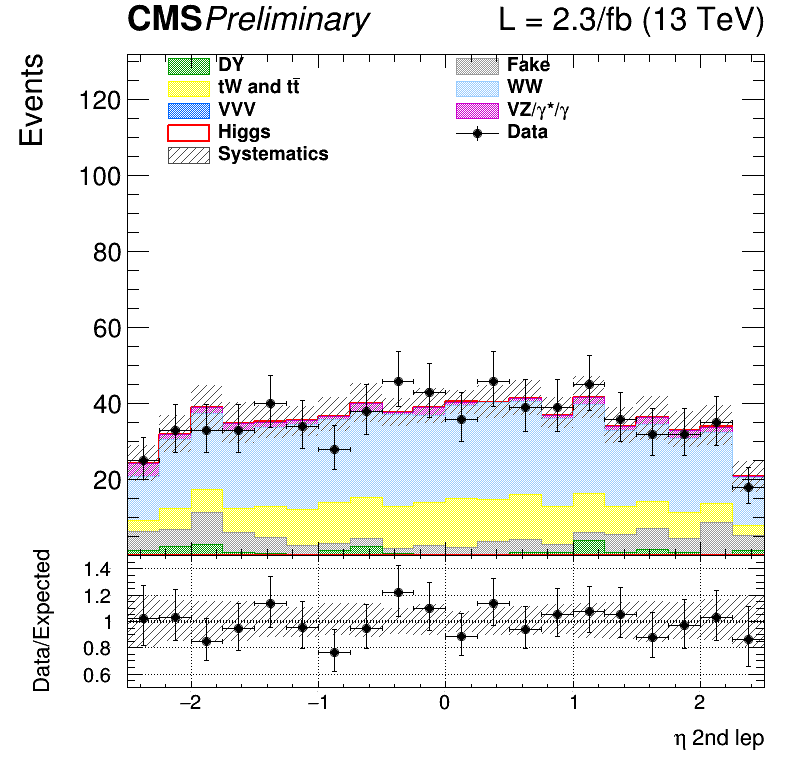
\includegraphics[width=0.45\textwidth]{images/13TeV/cratio_ww2l2v_13TeV_ww_of0j_eta2}
}\\
\subfigure[1 jet - $\pt^{\ell,2}$]{
  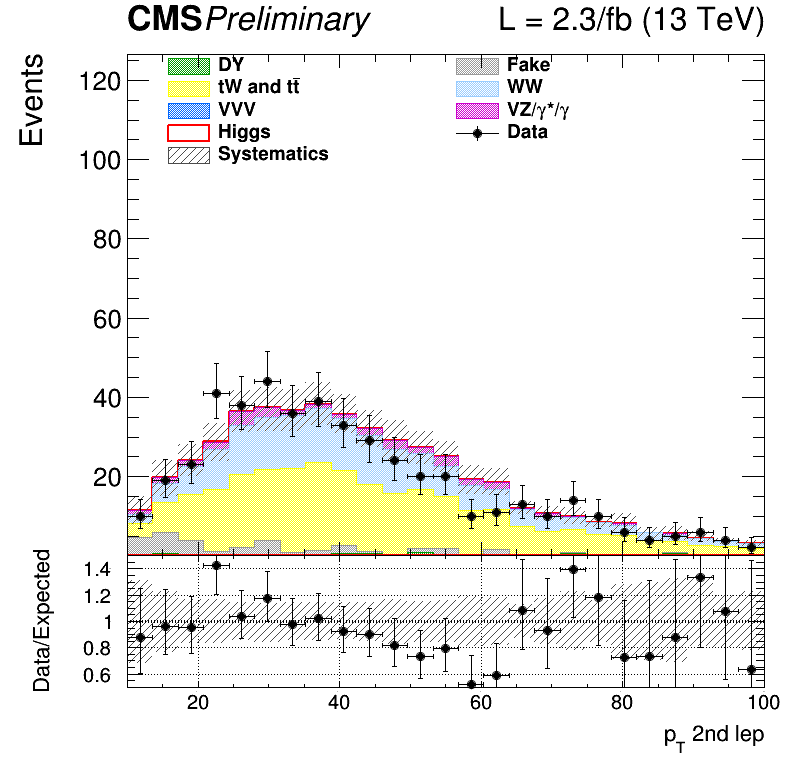
\includegraphics[width=0.45\textwidth]{images/13TeV/cratio_ww2l2v_13TeV_ww_of1j_pt2}
}
\subfigure[1 jet - $\eta^{\ell,2}$]{
  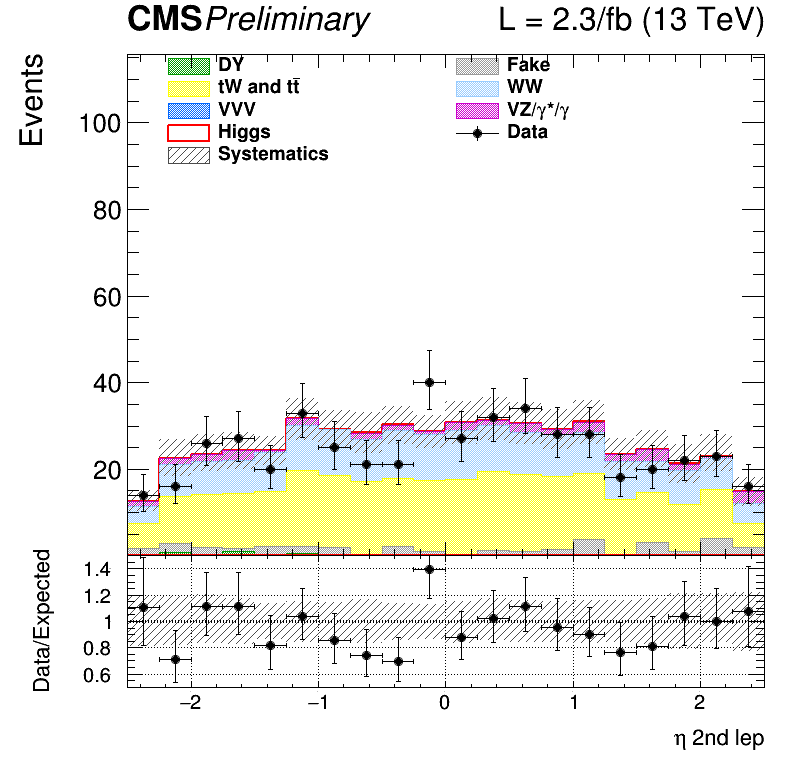
\includegraphics[width=0.45\textwidth]{images/13TeV/cratio_ww2l2v_13TeV_ww_of1j_eta2}
}
\caption{Distributions of \pt (left) and $\eta$ (right) of the subleading lepton in events with 0 jets (upper row) and 1 jet (bottom row), for the main backgrounds (stacked histograms), and for a SM Higgs boson signal with $m_\mathrm{H}=125$\GeV (superimposed and stacked red histogram)  after the analysis event selection.}\label{fig:distr2}
\end{figure}

\begin{figure}
\centering
\subfigure[0 jets - \MET]{
  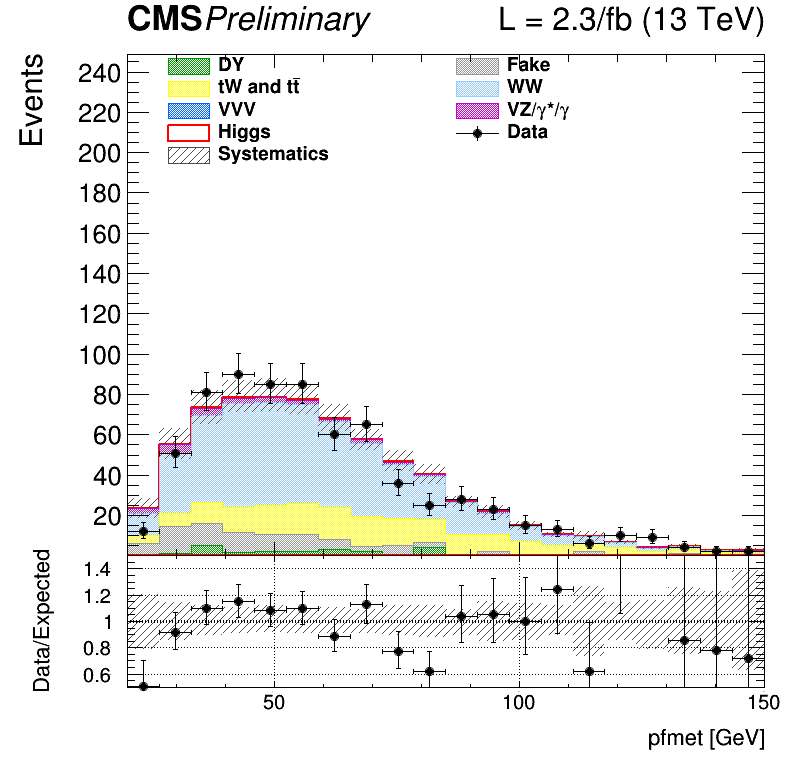
\includegraphics[width=0.45\textwidth]{images/13TeV/cratio_ww2l2v_13TeV_ww_of0j_met}
}
\subfigure[0 jets - \ptll]{
  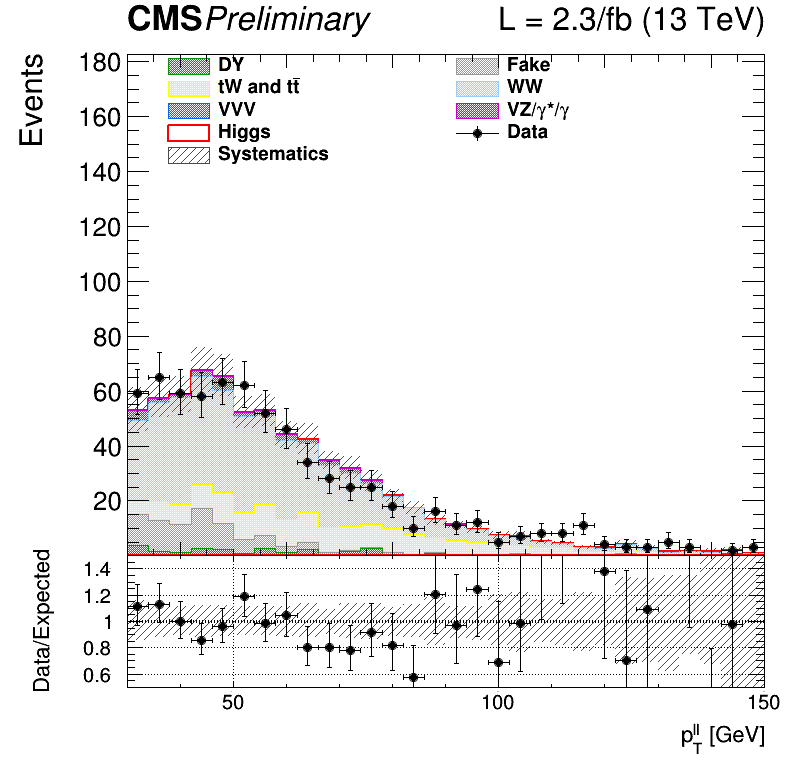
\includegraphics[width=0.45\textwidth]{images/13TeV/cratio_ww2l2v_13TeV_ww_of0j_ptll}
}\\
\subfigure[1 jet - \MET]{
  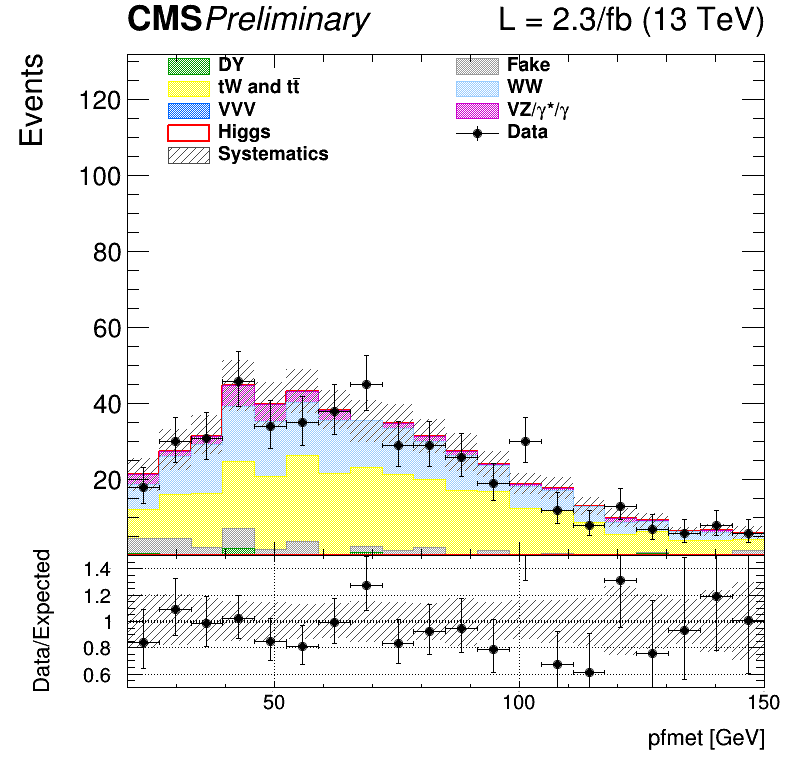
\includegraphics[width=0.45\textwidth]{images/13TeV/cratio_ww2l2v_13TeV_ww_of1j_met}
}
\subfigure[1 jet - \ptll]{
  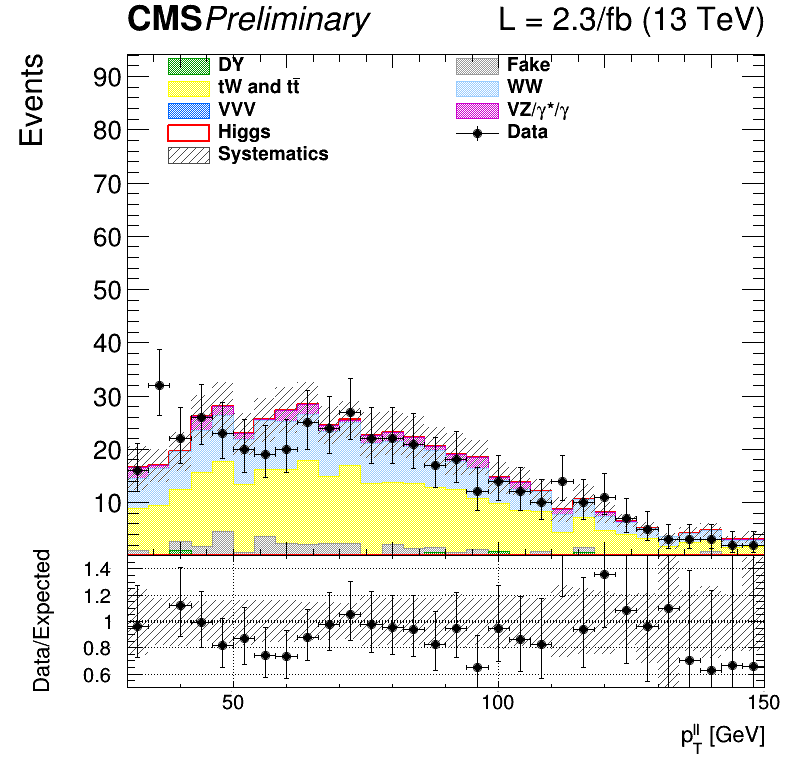
\includegraphics[width=0.45\textwidth]{images/13TeV/cratio_ww2l2v_13TeV_ww_of1j_ptll}
}
\caption{Distributions of \MET (left) and \ptll (right) in events with 0 jets (upper row) and 1 jet (bottom row), for the main backgrounds (stacked histograms), and for a SM Higgs boson signal with $m_\mathrm{H}=125$\GeV (superimposed and stacked red histogram) after the analysis event selection.}\label{fig:distr3}
\end{figure}

An additional categorization is applied in order to increase the signal sensitivity. The 0 ad 1 jets categories are further split according to the lepton flavour to e$\mu$ and $\mu$e, where the first lepton refers to the leading one. In this way an improvement of about 10\% in terms of signal significance can be achieved, exploiting the different W+jets background contribution in the two categories. Actually, this background is characterized by the presence of one jet misidentified as a lepton, and the probability for a jet to be misidentified as a muon is larger than as an electron.

\subsection{Signal extraction}

To extract the Higgs boson signal contribution in the four previously mentioned categories, a similar approach to the one used in the 8\TeV differential measurement (see Sec.~\ref{sec:SignalExtraction}) is pursued. The analysis is based on two-dimensional templates of \mll versus \mt to discriminate signal and background contributions. The \mll template is defined using 5 bins from $\mll=10$\GeV up to $\mll=110$\GeV, while for the \mt template 7 bins are defined in the range $60\GeV < \mt < 200$\GeV. The phase space with $\mt<60$\GeV is used as an orthogonal control region to extract the normalization of the \dytt background. A binned maximum likelihood fit to the signal and background two-dimensional templates is performed to extract the signal strength in the four categories.

The statistical methodology used to interpret the data and combine the results from the independent 0 and 1 jets categories in the e$\mu$ and $\mu$e final states has been developed by the ATLAS and CMS collaborations in the context of the LHC Higgs Combination Group~\cite{CMS-NOTE-2011-005,Khachatryan:2014jba}.
The number of events in each category and in each bin of the two-dimensional template is modelled as a Poisson random variable, with a mean value given by the sum of the contributions from all the processes under consideration. Systematic uncertainties are represented by individual nuisance parameters with log-normal distributions. The uncertainties affect the overall normalization of signal and backgrounds, as well as their (\mll, \mt) shape. Correlations between systematic uncertainties in different categories are taken into account. 













\section{Background estimation}\label{chap5:backgrounds}

The main background processes affecting the analysis signature, nonresonant WW production and top quark processes, are estimated using data. Backgrounds arising from an experimental misidentification of the objects, such as W+jets, are estimated using data as well. The other minor backgrounds are generally estimated directly from simulation as described in the following sections.

\subsection{WW background}

The quark-induced WW background is simulated with NLO accuracy in perturbative QCD, and the transverse momentum of the diboson system is reweighted to match the NNLO+NNLL accuracy from theoretical calculations~\cite{Meade:2014fca,Jaiswal:2014yba}. However, given the large uncertainties in the jet multiplicity distribution associated to this process, the normalization of this background is measured from data separately for the 0 and 1 jets categories. The normalization scale factors are extracted directly from the fit, leaving the WW normalization free to float separately in the two jet multiplicity categories. An orthogonal control region for the WW background normalization estimation is not needed in this case, owing to the different (\mll, \mt) shape for signal and background.

The gluon-induced WW production is subdominant with respect to the quark-induced production, and its shape and normalization are taken from simulation, scaling the cross section to the theoretical NLO accuracy prediction~\cite{Caola:2015rqy}.

\subsection{Top quark background}

As explained in Sec.~\ref{chap5:analysis_strategy}, the production of top quark pairs represents one of the dominant backgrounds in this analysis given its large cross section and a final state similar to the signal process. A b-jet veto, based on the cMVAv2 b tagging algorithm, is used to suppress this background and a reweighting procedure is applied to simulated events to correct for different b tagging efficiency in data and simulation.

The top quark background normalization is measured using data, defining a b-jets enriched control region by inverting the b-jet veto. More precisely, the b-jets enriched control region for the 0 jets category is defined with the same WW baseline selection but requiring at least one jet with $20<\pt<30$\GeV to be identified as a b-jet and no other jets with $\pt > 30$\GeV. For the 1 jet category, the b-jets enriched region is defined requiring exactly one jet with $\pt>30$\GeV identified as a b-jet.
To reduce other backgrounds in these two regions, the dilepton mass has to be greater than 50\GeV. Distributions of the \mll and \mt variables in the b-jets enriched control regions after applying the data driven estimation are shown in Figure~\ref{fig:TopCtrl125} for the 0 and 1 jets categories separately.

The top quark background normalization is constrained during the fit procedure separately in the two jet categories by means of the control regions defined above, which are treated in the fit as two additional categories. 

\begin{figure}[htb]
\centering
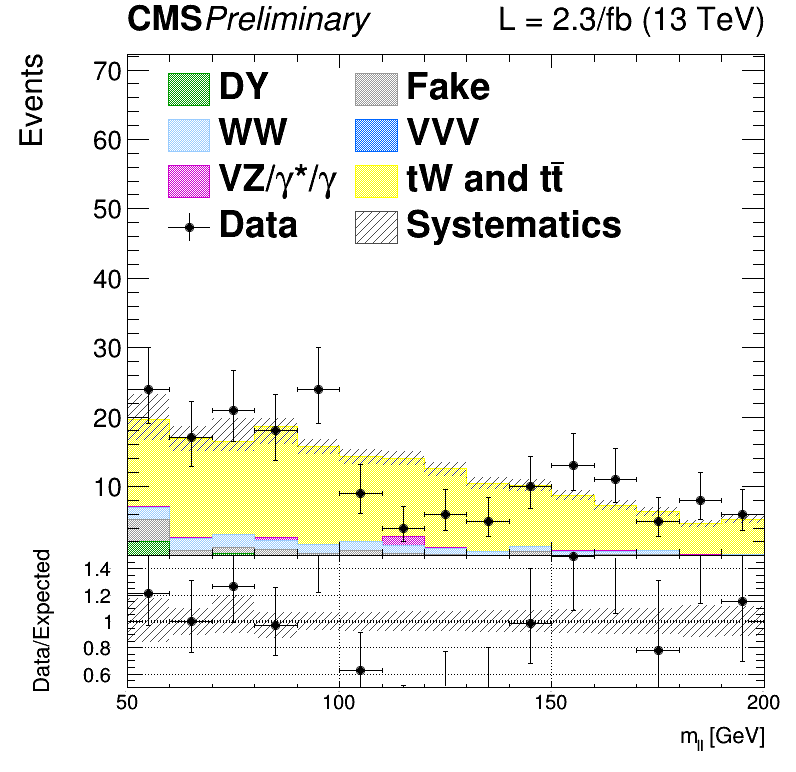
\includegraphics[width=0.45\textwidth]{images/13TeV/cratio_hww2l2v_13TeV_top_of0j_mll.png}
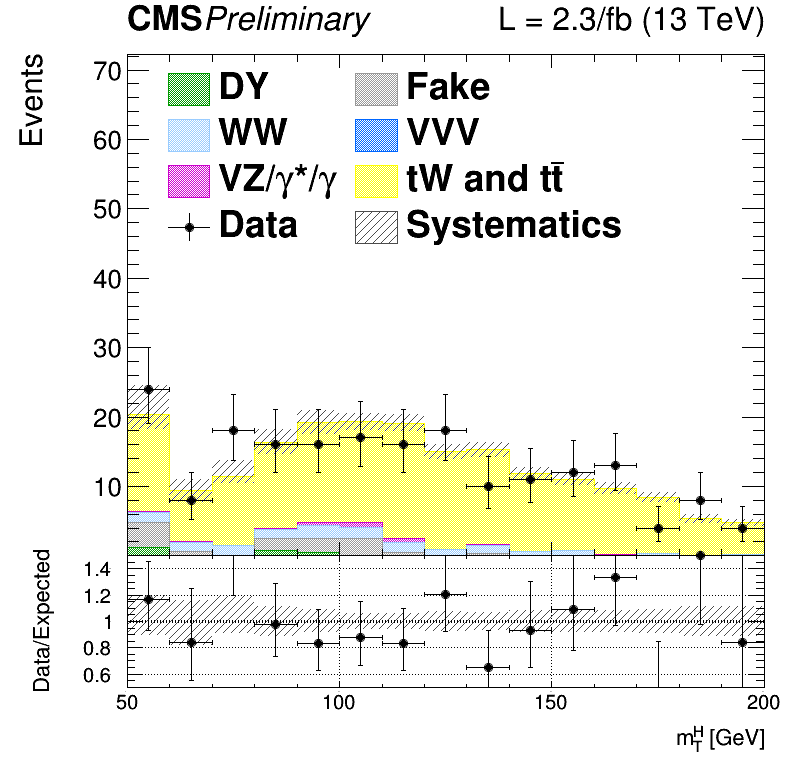
\includegraphics[width=0.45\textwidth]{images/13TeV/cratio_hww2l2v_13TeV_top_of0j_mth.png}
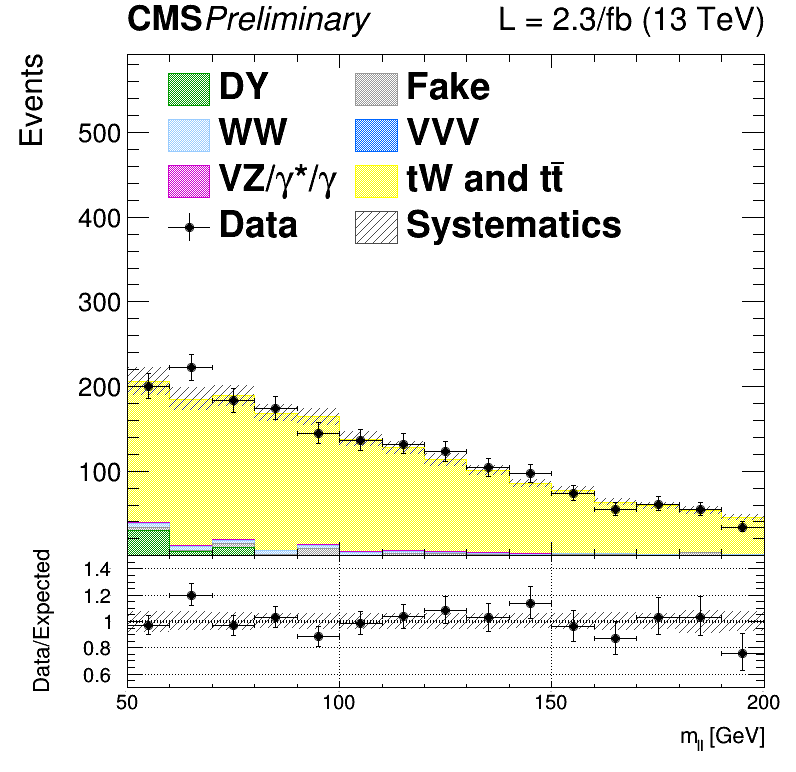
\includegraphics[width=0.45\textwidth]{images/13TeV/cratio_hww2l2v_13TeV_top_of1j_mll.png}
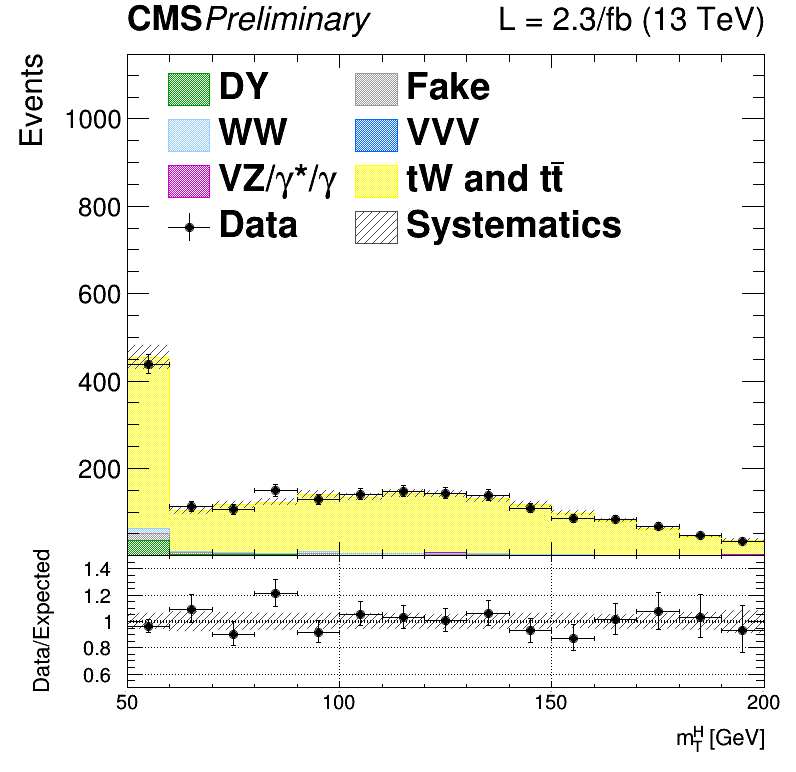
\includegraphics[width=0.45\textwidth]{images/13TeV/cratio_hww2l2v_13TeV_top_of1j_mth.png}
\caption{
Distributions of \mll (left) and \mt (right) for events with 0 jets (top) and 1 jet (bottom) in the b-jets enriched phase space. Scale factors estimated from data are applied.%The first (last) bin includes underflows (overflows).
}
\label{fig:TopCtrl125}
\end{figure}

\subsection{W+jets background}

One of the primary source belonging to this category arises from the misidentification of leptons in W+jets (also known as ``Fake'' or ``jet-induced'') processes in the 0 jets category. Also, semileptonic \ttbar decays contribute especially for higher jet multiplicities. Multijet production and hadronic \ttbar decays are also taken into account, despite their smaller contribution.

This background is fully estimated using data, with the technique described in Sec.~\ref{sec:wjetsbkg}. To check the agreement of the background estimated in this way with data, a control sample enriched in Fake events is defined. The events in the control sample are selected applying the WW baseline requirements but requesting an e$\mu$ pair with same charge, significantly suppressing the WW and \ttbar processes. The \mll distributions in this control region for the 0 and 1 jets categories are shown in Fig.~\ref{fig:13TeVsamesign}. From this cross-check a global normalization factor of 0.8 is derived in both categories and applied to the Fake background.

\begin{figure}[htb]
\centering
    \subfigure[0 jets]{
    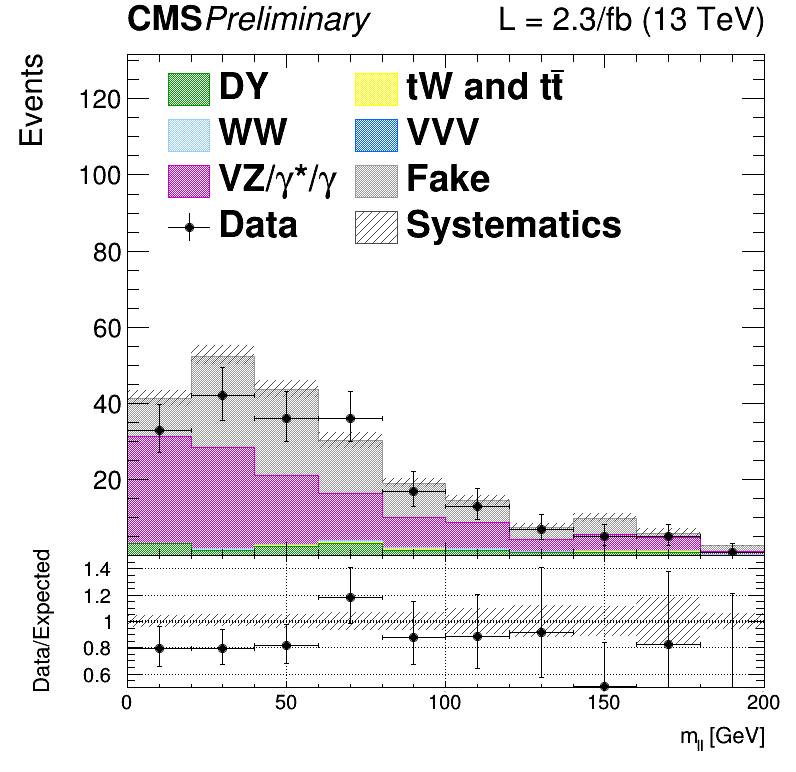
\includegraphics[width=0.45\textwidth]{images/13TeV/cratio_hww2l2v_13TeV_ss_of0j_mll.png}
    }
    \subfigure[1 jet]{
    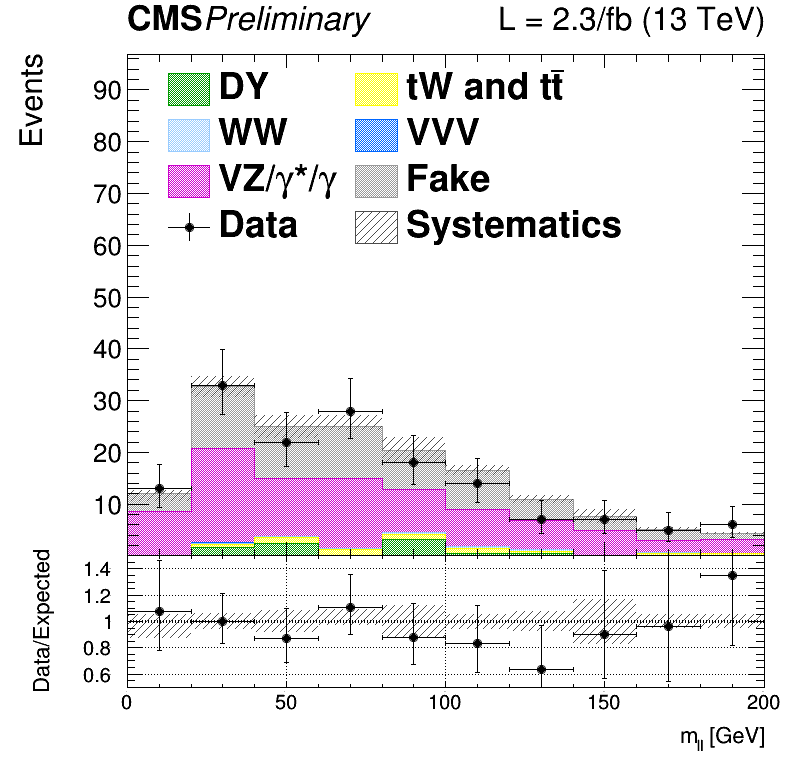
\includegraphics[width=0.45\textwidth]{images/13TeV/cratio_hww2l2v_13TeV_ss_of1j_mll.png}
    }
    \caption{
         Control plots for \mll in a Fake enriched phase space for events with 0 and 1 jet with $\pt > 30$\GeV, in e$\mu$ final state. The normalization factor is not applied.
         }\label{fig:13TeVsamesign}
\end{figure}

\subsection[\dytt background]{\boldmath$\dytt$ background}\label{chap5:DYbackground}

This background contributes to the analysis phase space because of the $\mathrm{Z}/\gamma^*$ decays to a pair of $\tau$ leptons, which consequently decay to an e$\mu$ pair. This background process is predominant in the low \mt region, which is used as an orthogonal control region to determine the background normalization in the 0 and 1 jets categories. In particular, this control region is defined by selecting events with $\mt < 60$\GeV and $30\GeV < \mll < 80$\GeV. The \mll distributions in the control regions for the 0 and 1 jets categories are shown in Fig.~\ref{fig:13TeVDYtt}.

As for the top quark background, the normalization of this background is constrained directly in the fit by means of the two control regions, which are treated as two additional categories.

The kinematics of this background is taken from simulation, after reweighting the Z boson \pt spectrum to match the observed distribution in data. In fact, this variable is not well reproduced by the MC generator used for simulating this process, especially in the bulk of the distribution. The discrepancy is ascribed to the missing contribution from resummed calculations.

\begin{figure}[htb]
\centering
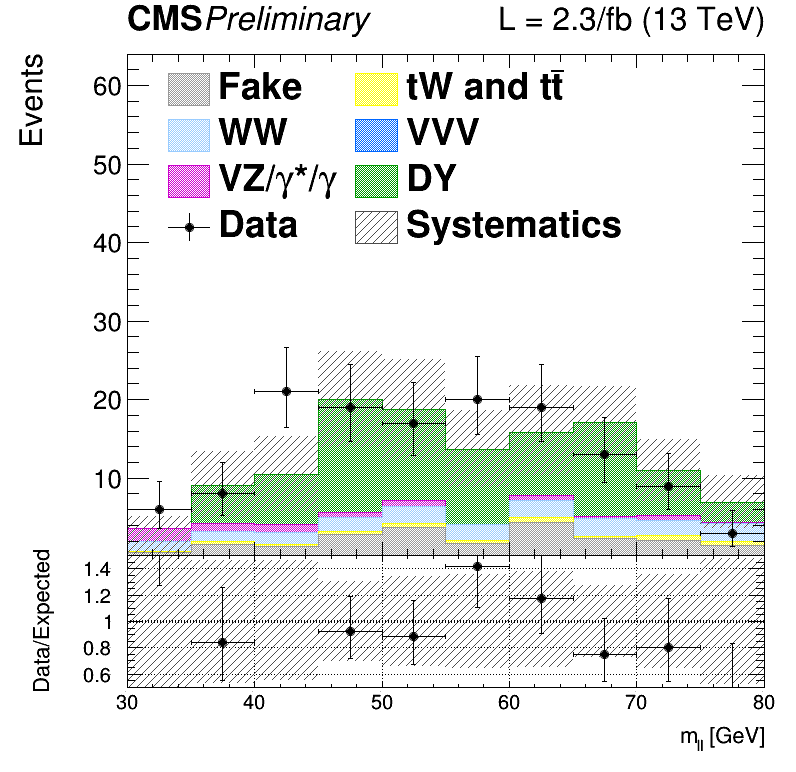
\includegraphics[width=0.45\textwidth]{images/13TeV/cratio_hww2l2v_13TeV_dytt_of0j_mll.png}
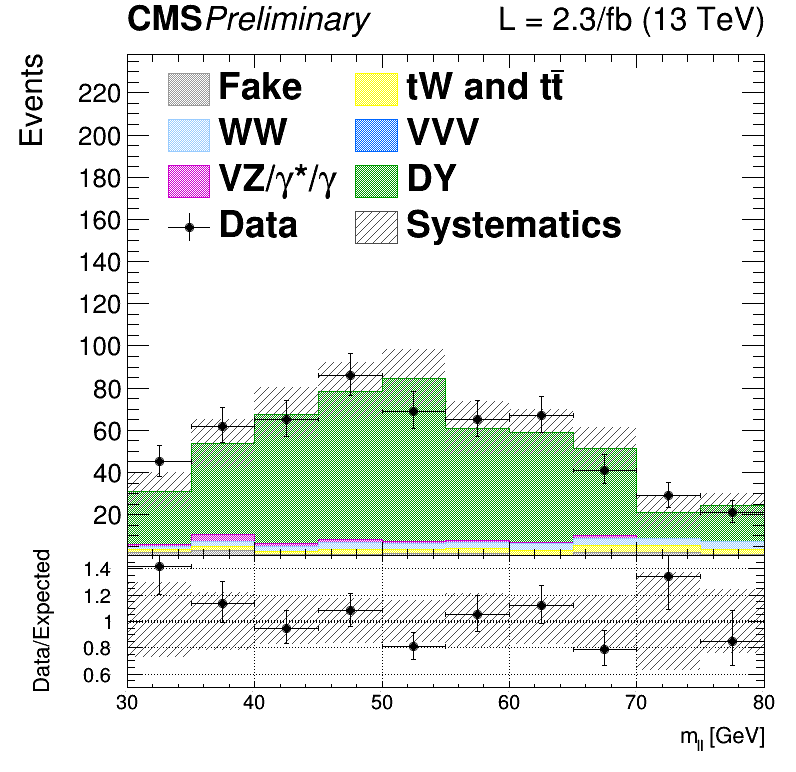
\includegraphics[width=0.45\textwidth]{images/13TeV/cratio_hww2l2v_13TeV_dytt_of1j_mll.png}
\caption{
Distributions of \mll for events with 0 jets (left) and 1 jet (right) in the \dytt enriched control region. Scale factors estimated from data are applied.}
\label{fig:13TeVDYtt}
\end{figure}

\subsection{Other backgrounds}\label{chap5:otherBackgrounds}

The W$\gamma^*$ and the WZ electroweak processes can be gathered in the same physical process, although the final state kinematics is rather different. In particular, the invariant mass of the leptons arising from the $\gamma^*$ decays is generally below 4\GeV, while the leptons from the Z boson decay are characterized by a larger invariant mass. Another background that may be experimentally identical to those is the W$\gamma$ production, where a real photon produced in association with a W boson undergoes a photon conversion to leptons due to the interaction with the material of the silicon tracker.

All these backgrounds may contribute to the signal phase space whenever one of the three leptons escape from the detector acceptance or is not identified. The shape and cross section of these backgrounds are taken from simulation. The only exception is the normalization of the W$\gamma^*$ background, being this process dominant in the low \mll region, which is scaled to data defining a proper control region. The control region is defined selecting events with three isolated muons, with $\pt > 10$, 5 and 3\GeV for the first three leading muons, respectively. The selection is further defined by requiring $\MET < 25\GeV$. The pair of muons with the smallest invariant mass is taken as coming from the $\gamma^{*}$ decay. The $k$-factor measured in data for this background is $1.98\pm0.54$.

All remaining backgrounds from diboson and triboson production, which are of minor importance in the analysis phase space, are normalized according to their expected theoretical cross sections.






\section{Systematic uncertainties}\label{chap5:systs}

The systematic uncertainties affecting this measurement can be divided into three categories: the uncertainties on the background estimation, experimental uncertainties and theoretical uncertainties.

The first category includes the uncertainties related to the background normalization and shape. For the non-resonant WW production the shape is taken from simulation. The input normalization to the fit is set to the expected value from simulation, and an unconstrained nuisance parameter with a flat distribution is associated to this number. This is done separately for the two jet categories.

The top quark background shape is taken from simulation after correcting for the b tagging scale factors. An uncertainty due to these scale factors is included and affects both the normalization and the shape of the top quark background. The uncertainties on the normalization are treated similarly to the WW background case, but constraining the corresponding nuisances by means of the two control regions orthogonal to the signal phase space. A similar procedure is used for the DY background.

Effects due to experimental uncertainties are studied by applying a scaling and smearing of
certain variables related to the physics objects, e.g. the \pt of the leptons, followed by a subsequent recalculation of all the correlated variables. This is done for simulation, to account for possible systematic mismodeling.

All experimental sources, except luminosity, are treated both as normalization and shape uncertainties, and are correlated among the signal and background processes and all the categories. The following experimental uncertainties are considered:
\begin{itemize}
\item the uncertainty determined by the CMS online luminosity monitoring, 2.7\% for the first data collected at $\sqrt{s}=13$\TeV;
\item the acceptance uncertainty associated with the combination of single and double lepton triggers, which is 2\%;
\item the lepton reconstruction and identification efficiencies uncertainties, that are in the range 0.5-5\% for electrons and 1-7\% for muons depending on \pt and $\eta$;
\item the muon momentum and electron energy scale and resolution uncertainties, that amount to 0.01-0.5\% for electrons and 0.5-1.5\% for muons depending on \pt and $\eta$;
\item the jet energy scale uncertainties, that vary between 1-11\% depending on the \pt and $\eta$ of the jet;
\item the \MET resolution uncertainty, that is taken into account by propagating the corresponding uncertainties on the leptons and jets;
\item the scale factors correcting the b tagging efficiency and mistagging rate, that are varied within their uncertainties. This systematic uncertainty is anticorrelated between the top control regions and the other ones.
\end{itemize}

The uncertainties in the signal and background production rates due
to theoretical uncertainties include several components, which are assumed to be
independent: the PDFs and $\alpha_{s}$, the underlying event and parton shower model,
and the effect of missing higher-order corrections via variations of the renormalization
and factorization scales.

The effects of the variation of PDFs, $\alpha_s$ and renormalization/factorization QCD scales, mainly affect the signal processes, being the most important backgrounds estimated using data driven techniques. However, the uncertainties on minor backgrounds that are estimated from simulation are taken into account. These uncertainties are split in the uncertainties on the cross section, which are computed by the LHC cross section working group~\cite{YRtmp}, and on the selection efficiency~\cite{Butterworth:2015oua}. The PDFs and $\alpha_{s}$ signal cross section normalization uncertainties are $^{+7.4\%}_{-7.9\%}$ and $^{+7.1\%}_{-6.0\%}$ for ggH and $\pm 0.7\%$ and $\pm 3.2\%$ for VBF Higgs production mechanism. The PDFs and $\alpha_{s}$ acceptance uncertainties are less than 1\% for gluon- and quark-induced processes. The effect of the QCD scales variation on the selection efficiency is around 1-3\% depending on the specific process. To estimate these uncertainties, the events are reweighted according to different QCD scales or different PDF sets and the selection efficiency is recomputed each time. For the QCD scale uncertainty the maximum variation with respect to the nominal value is taken as the uncertainty. For the case of PDF and $\alpha_s$ uncertainties, the distribution of the selection efficiency is built taking into account all the replicas in the NNPDF3.0 set and the uncertainty is estimated as the standard deviation of that distribution.

In addition, the categorization of events based on jet multiplicity introduces additional uncertainties on the ggH production mode related to missing higher order corrections. These uncertainties are evaluated following the prescription described in Sec.~\cite{subsec:stewart-tackman} and correspond to 5.6\% for the 0-jet and 13\% for the 1-jet bin categories.

The underlying event uncertainty is estimated by comparing two different \textsc{pythia 8} tunes,
while parton shower modelling uncertainty is estimated by comparing samples interfaced
with the \textsc{pythia 8} and \textsc{herwig++} parton shower programs. 
The effect on the ggH (VBF) signal expected yield is about 5\% (5\%) for the \textsc{pythia 8} tune variation and about 7\% (10\%) for the parton shower description.

Other specific theoretical uncertainties are associated to some backgrounds. An uncertainty on the ratio of the \ttbar and tW cross sections is included. Indeed, these two processes are characterized by a different number of b-jets in the final state (2 b-jets for \ttbar and 1 for tW) and the b-veto acts differently for the two. A variation of the relative ratio of the cross sections can thus cause a migration of events from the 0 to the 1 jet categories and viceversa. The corresponding uncertainty is of 8\%, according to the theoretical cross section calculations~\cite{topxsec,singletop}.

The $\mathrm{gg}\to\mathrm{WW}$ background LO cross section predicted by the \textsc{mcfm} generator is scaled to the NLO calculation, applying a k-factor of 1.4 with an uncertainty of 15\%~\cite{Caola:2015rqy}. The interference term between the $\mathrm{gg}\to\mathrm{WW}$ and the ggH signal is also included and simulated with LO accuracy using \textsc{mcfm}. The k-factor to scale the interference term is 1.87, given by the geometrical average of the LO to NNLO gg$\to$H$\to$WW scale factor (2.5) and the LO to NLO $\mathrm{gg}\to\mathrm{WW}$ scale factor (1.4). The uncertainty on this value is estimated as the maximum variation with respect to the two scale factors mentioned above, and is found to be of 25\%. Anyway, with the current amount of integrated luminosity, the interference contribution is found to be negligible.

For what the $\mathrm{qq}\to\mathrm{WW}$ background shape is concerned, an uncertainty related to the diboson \pt reweighting is evaluated varying the renormalization, factorization and resummation QCD scales.

Finally, the uncertainties due to the limited statistical accuracy of the MC simulations are also taken into account, including an independent uncertainty for each bin of the two-dimensional distribution, and for each category. The uncertainty for a certain bin and process is given by the standard deviation of the Poisson distribution with mean corresponding to the number of MC events in that bin.


 

\section{Results}\label{chap5:results}

Distributions of the \mll and \mt variables after the full analysis selection are shown in Fig.~\ref{fig:mllandmt} for the 0 and 1 jets categories separately, but merging the e$\mu$ and $\mu$e final states together.

\begin{figure}
\centering
\subfigure[0 jets - \mll]{
  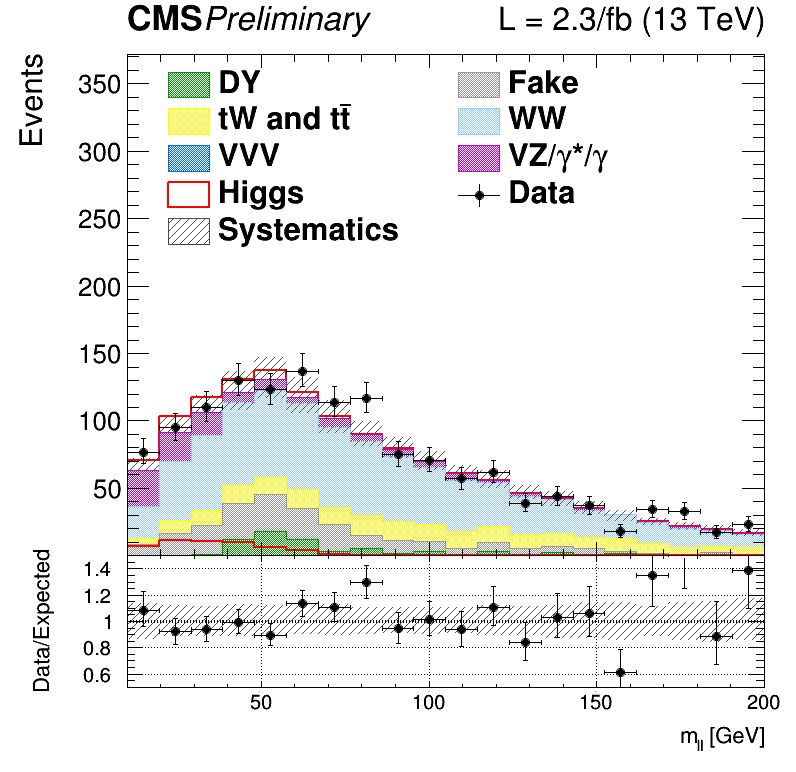
\includegraphics[width=0.45\textwidth]{images/13TeV/cratio_hww2l2v_13TeV_of0j_mll}
}
\subfigure[0 jets - \mt]{
  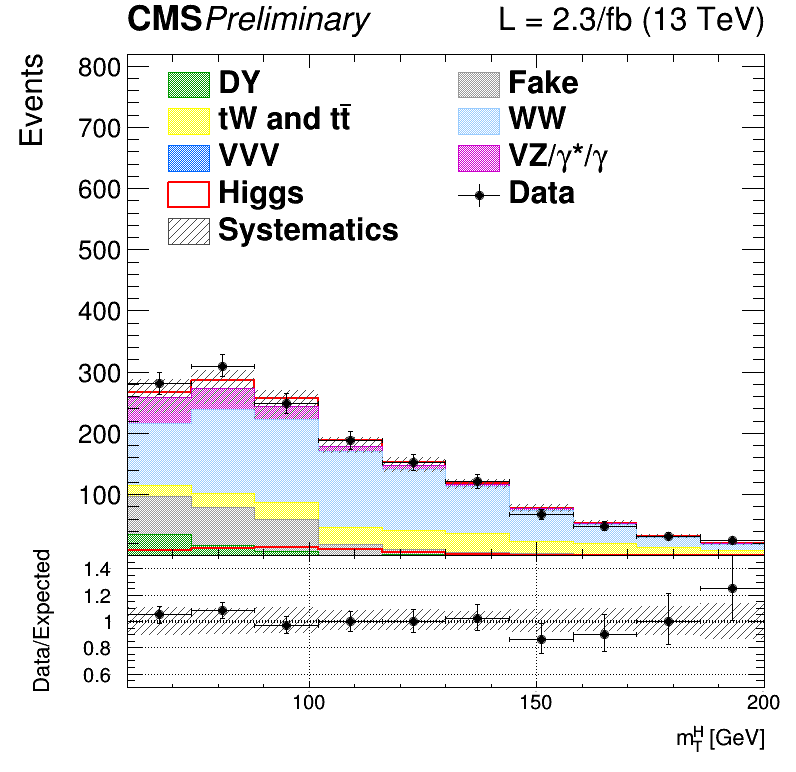
\includegraphics[width=0.45\textwidth]{images/13TeV/cratio_hww2l2v_13TeV_of0j_mth}
}\\
\subfigure[1 jet - \mll]{
  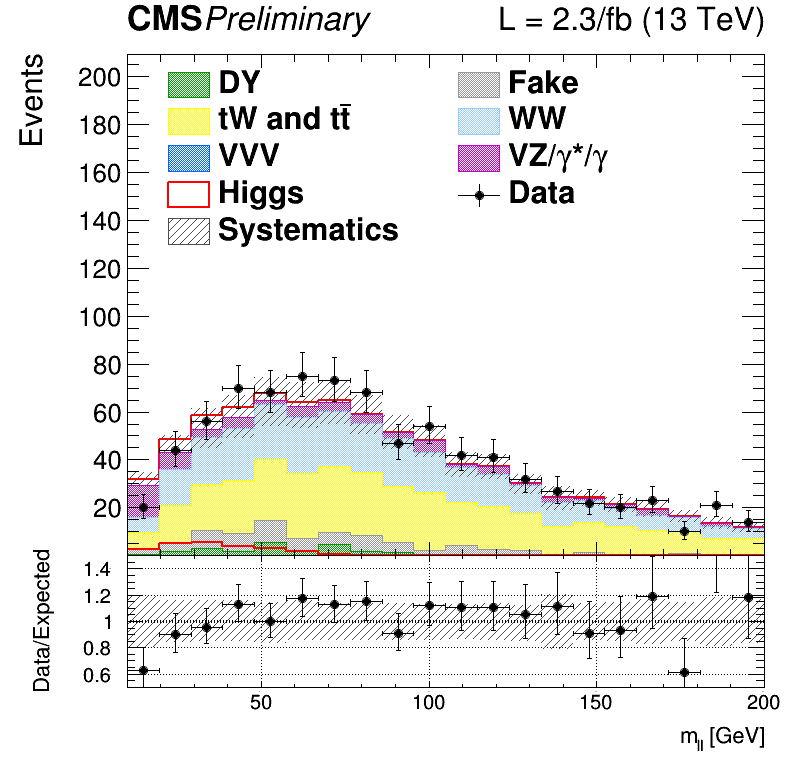
\includegraphics[width=0.45\textwidth]{images/13TeV/cratio_hww2l2v_13TeV_of1j_mll}
}
\subfigure[1 jet - \mt]{
  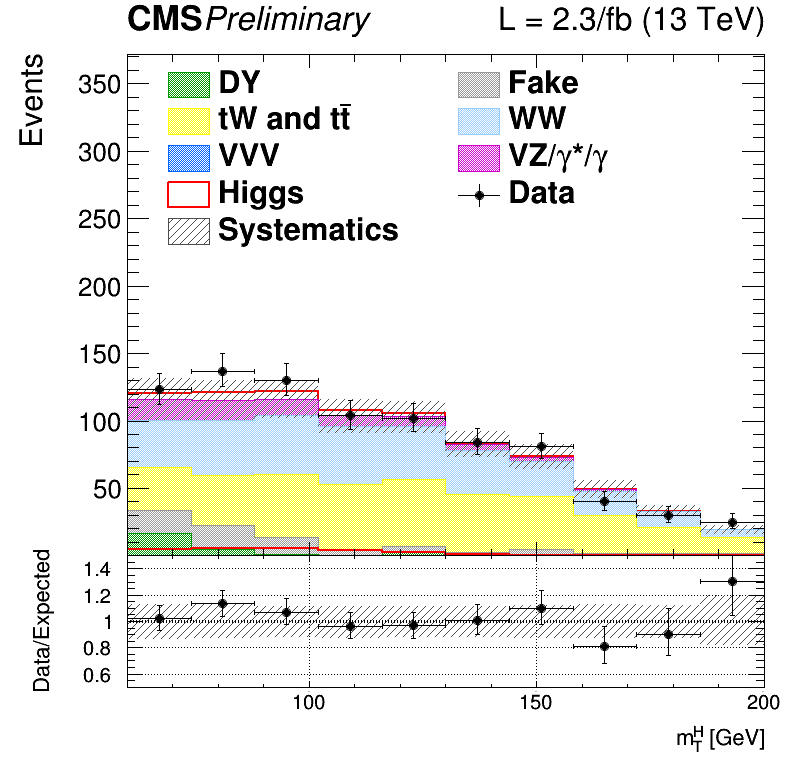
\includegraphics[width=0.45\textwidth]{images/13TeV/cratio_hww2l2v_13TeV_of1j_mth}
}
\caption{Distributions of \mll (left) and \mt (right) for events with 0 jets (upper row) and 1 jet (lower row), for the main backgrounds (stacked histograms), and for a SM Higgs boson signal with $m_\mathrm{H}=125$\GeV (superimposed and stacked red histogram) after the analysis event selections. The simulation of the WW background is normalized to data.}\label{fig:mllandmt}
\end{figure}

\begin{table}[!htb]
\caption{Observed and expected significance and signal strength for the SM Higgs boson with $m_{\rm H}=125$\GeV in the 0 and 1 jets categories. The $\mu$e and e$\mu$ configurations are shown separately.}\label{tab:13TeVsignif}
\begin{center}
\begin{tabular}{lccc}
\toprule
Category  &  Expected significance      &  Observed  significance    &  $\sigma/\sigma_{SM}$     \\
\midrule
0 jet  $\mu$e   &     1.1        &  1.3        &  1.13 $_{-0.9}^{+0.9}$             \\ [5pt]   

0 jet  e$\mu$   &     1.3        &  0.4        &  0.33 $_{-0.7}^{+0.7}$             \\ [5pt]   

1 jet  $\mu$e   &     0.8        &  0          &  -0.11$_{-1.7}^{+0.5}$                 \\ [5pt] 

1 jet  e$\mu$   &     0.9        &  0          &  -0.54$_{-1.4}^{+1.4}$                 \\ [5pt] 

\midrule 

0 jet           &     1.6        &  1.3       &  0.71$_{-0.5}^{+0.6}$             \\ [5pt]  

1 jet           &     1.2        &  0         &  -0.56$_{-1.0}^{+1.0}$                \\ [5pt]  

\midrule 
Combination     &     2.0        &  0.7       &  0.33$_{-0.5}^{+0.5}$              \\ [5pt]  
\bottomrule
\end{tabular}
\end{center}
\end{table}

The expected and observed signal significances are shown in Table~\ref{tab:13TeVsignif} for all the categories. Also, the observed signal strengths and the corresponding uncertainties are shown. The best fit signal strength obtained combining all the categories together is found to be $0.3^{+0.5}_{-0.5}$, corresponding to an observed significance of $0.7\,\sigma$, to be compared with the expected significance of $2.0\,\sigma$ for a Higgs boson mass of 125\GeV.

The measurement is dominated by the statistical uncertainties on data. The main systematic contributions affecting the uncertainty on the signal strength arise from the Fake background estimation, lepton identification and isolation, luminosity, b tagging scale factors, WW and \ttbar background normalization and other minor backgrounds. The uncertainty on the data driven backgrounds mainly arise from the limited data statistics in the control regions used for measuring the normalization.
A summary of the most important systematic uncertainties and their effect on the signal strength uncertainty is illustrated in Table~\ref{tab:mu_syst}.

\begin{table}[htb]
\caption{Main systematic sources and their contribution to the signal strength uncertainty ($\Delta\mu/\mu$).}\label{tab:mu_syst}
\begin{center}
\begin{tabular}{lc}
\toprule
Systematic uncertainty  &   $\Delta\mu/\mu$\\
\midrule
Fake background estimation & 25\% \\
Lepton identification and isolation & 20\% \\
W$\gamma^*$ background cross section & 12\% \\
WW and \ttbar data driven normalization & 10\% \\
Luminosity & 8\% \\
b tagging scale factors & 6\% \\
Lepton scale and resolution & 3\% \\
\bottomrule
\end{tabular}
\end{center}
\end{table}

